\documentclass[lettersize,journal]{IEEEtran}
\usepackage{amsmath,amsfonts}
\usepackage{algorithmic}
\usepackage{algorithm}
\usepackage{array}
\usepackage[caption=false,font=normalsize,labelfont=sf,textfont=sf]{subfig}
\usepackage{textcomp}
\usepackage{stfloats}
\usepackage{url}
\usepackage{verbatim}
\usepackage{graphicx}
\usepackage{cite}
\usepackage{booktabs}
\usepackage{xcolor}
\usepackage{tabularx}
\usepackage{adjustbox}
% define a table width variable used by some tabular* environments
\newlength{\tblwidth}
\setlength{\tblwidth}{\linewidth}
% theorem environments
\usepackage{amsthm}
\newtheorem{theorem}{Theorem}
\newtheorem{definition}{Definition}
\newtheorem{assumption}{Assumption}
\newtheorem{problem}{Problem}
\newtheorem{lemma}{Lemma}
\newtheorem{corollary}{Corollary}
% simple macros to support pseudocode keywords used in the paper
\providecommand{\UPON}[1]{\STATE \textbf{upon} #1}
\providecommand{\ENDUPON}{}
% algorithmic already provides \RETURN; avoid redefining it
\hyphenation{op-tical net-works semi-conduc-tor IEEE-Xplore}
% updated with editorial comments 8/9/2021

\begin{document}

\title{STLC: Spatiotemporal Localized Consensus with Adaptive Trust for Scalable Byzantine Fault Tolerance in Industrial Cyber-Physical Systems}

\author{Qi~Yu\IEEEauthorrefmark{1}\IEEEauthorrefmark{3},~\IEEEmembership{Member,~IEEE,}
	Li~Wei\IEEEauthorrefmark{2}\IEEEauthorrefmark{3},~\IEEEmembership{Member,~IEEE,}
	
\IEEEauthorblockA{\IEEEauthorrefmark{1}School of Cyber Science and Engineering, Southeast University, Nanjing 211189, PR China}

\IEEEauthorblockA{\IEEEauthorrefmark{2}School of Computer Science and Engineering, Southeast University, Nanjing 211189, PR China}

\IEEEauthorblockA{\IEEEauthorrefmark{3}Key Laboratory of Computer Network and Information Integration (Southeast University), MOE, Southeast University, Nanjing 211189, PR China} 

\thanks{Q. Yu is with the School of Cyber Science and Engineering, Southeast University, Nanjing 211189, PR China.}
\thanks{W. Li is with the School of Computer Science and Engineering, Southeast University, Nanjing 211189, PR China}
\thanks{Manuscript received Mar 26, 2026; %revised Mar 26, 2026.
Corresponding author: W. Li (email: xchlw@seu.edu.cn).}
}

% The paper headers
\markboth{IEEE Transactions on Automation Science and Engineering,~Vol.~14, No.~8, August~2026}%
{Qi \MakeLowercase{\textit{et al.}}: STLC: Spatiotemporal Localized Consensus with Adaptive Trust for Scalable Byzantine Fault Tolerance in Industrial Cyber-Physical Systems}

\IEEEpubid{0000--0000/00\$00.00~\copyright~2026 IEEE}
% Remember, if you use this you must call \IEEEpubidadjcol in the second
% column for its text to clear the IEEEpubid mark.

\maketitle

\begin{abstract}
Traditional Practical Byzantine Fault Tolerance (PBFT) protocols require all nodes to
participate in every consensus round, resulting in $O(N^2)$ communication
complexity that limits scalability and becomes prohibitive in large-scale industrial multi-agent
systems. This paper introduces STLC (Spatiotemporal Localized Consensus with Adaptive Trust), a novel framework exploiting
spatiotemporal context and adaptive trust weights to achieve efficient
Byzantine consensus through dynamic consensus locality. We formalize
Dynamic Consensus Locality Theory, proving that consensus restricted to
task-coupled domains of size $k$ achieves equivalent safety and
liveness as global consensus while reducing complexity to $O(k^2)$. The
protocol integrates spatiotemporal validation for early malicious message
rejection, adaptive trust weights for rapid Byzantine isolation, and
replicated scheduler coordination for fault tolerance.
Experimental validation using CORE emulator (10-100 nodes) and Raspberry Pi testbed demonstrates 98.5\% message reduction versus
PBFT (1,770 $\to$ 27 messages for $k=3$, $|N|=30$), 60\% latency
improvement, 98\% detection rate for spatiotemporal attacks, and stable
performance independent of system size. STLC enables scalable and practical Byzantine
consensus for industrial deployments with 100+ agents on
resource-constrained hardware.
\end{abstract}

\begin{IEEEkeywords}
Scalable Byzantine Fault Tolerance, Byzantine consensus, Localized consensus, Task-coupled domains, Spatiotemporal validation, Industrial multi-agent systems, Adaptive trust, Industrial IoT
\end{IEEEkeywords}

\section{Introduction}
\label{sec:introduction}
\IEEEPARstart{B}{yzantine} Fault Tolerance (BFT) ensures reliable consensus in distributed systems where nodes may exhibit arbitrary malicious behavior~\cite{wu2024half, liu2024improved}. From blockchain networks~\cite{dotan2021survey} to industrial control systems~\cite{bhamare2020cybersecurity}, BFT mechanisms provide critical guarantees for coordinating autonomous agents under adversarial conditions. 
Consider a distributed system with $|N|$ nodes (agents). The fundamental challenge of Byzantine consensus is achieving agreement when up to $f < |N|/3$ nodes may behave maliciously—sending conflicting messages, withholding information, or deviating arbitrarily from the protocol. This $|N|/3$ bound is a theoretical necessity: Feldman et al.~\cite{feldman1997optimal} 
proved that no deterministic protocol can tolerate $f \geq |N|/3$ Byzantine nodes 
while guaranteeing agreement and termination.

Classical BFT protocols, exemplified by PBFT~\cite{bouhata2025byzantine}, achieve
strong consistency through multi-phase message exchanges but suffer from a critical
limitation: \textit{all $N$ nodes must participate in every consensus round
regardless of task relevance}. This \textbf{global participation requirement} limits scalability and leads
to $O(N^2)$ message complexity
—each of the $N$ nodes exchanges messages with all other nodes in multiple phases—becoming prohibitive in modern industrial systems with hundreds of heterogeneous agents and stringent real-time requirements~\cite{dhatterwal2022role, hady2025multi}.


\subsection{Motivation and Key Insight}

Modern smart factories and autonomous warehouses deploy large fleets of heterogeneous agents that collaborate to execute complex production workflows~\cite{vlachos2024smart}. Consider a typical material handling scenario in a smart factory with agents (Figure~\ref{fig:motivation}): 
\begin{itemize}
    \item \textbf{Automated Guided Vehicles (AGVs)} transport raw materials and semi-finished products between workstations, navigating autonomously using LiDAR and visual odometry.
    \item \textbf{Robot Arms (RAs)} perform assembly, welding, and quality inspection at fixed workstations, equipped with force sensors and vision systems.
    \item \textbf{Scheduling System (S)} coordinates task allocation, monitors production progress, and optimizes resource utilization.
\end{itemize}

\begin{figure*}[!t]
    \centering
    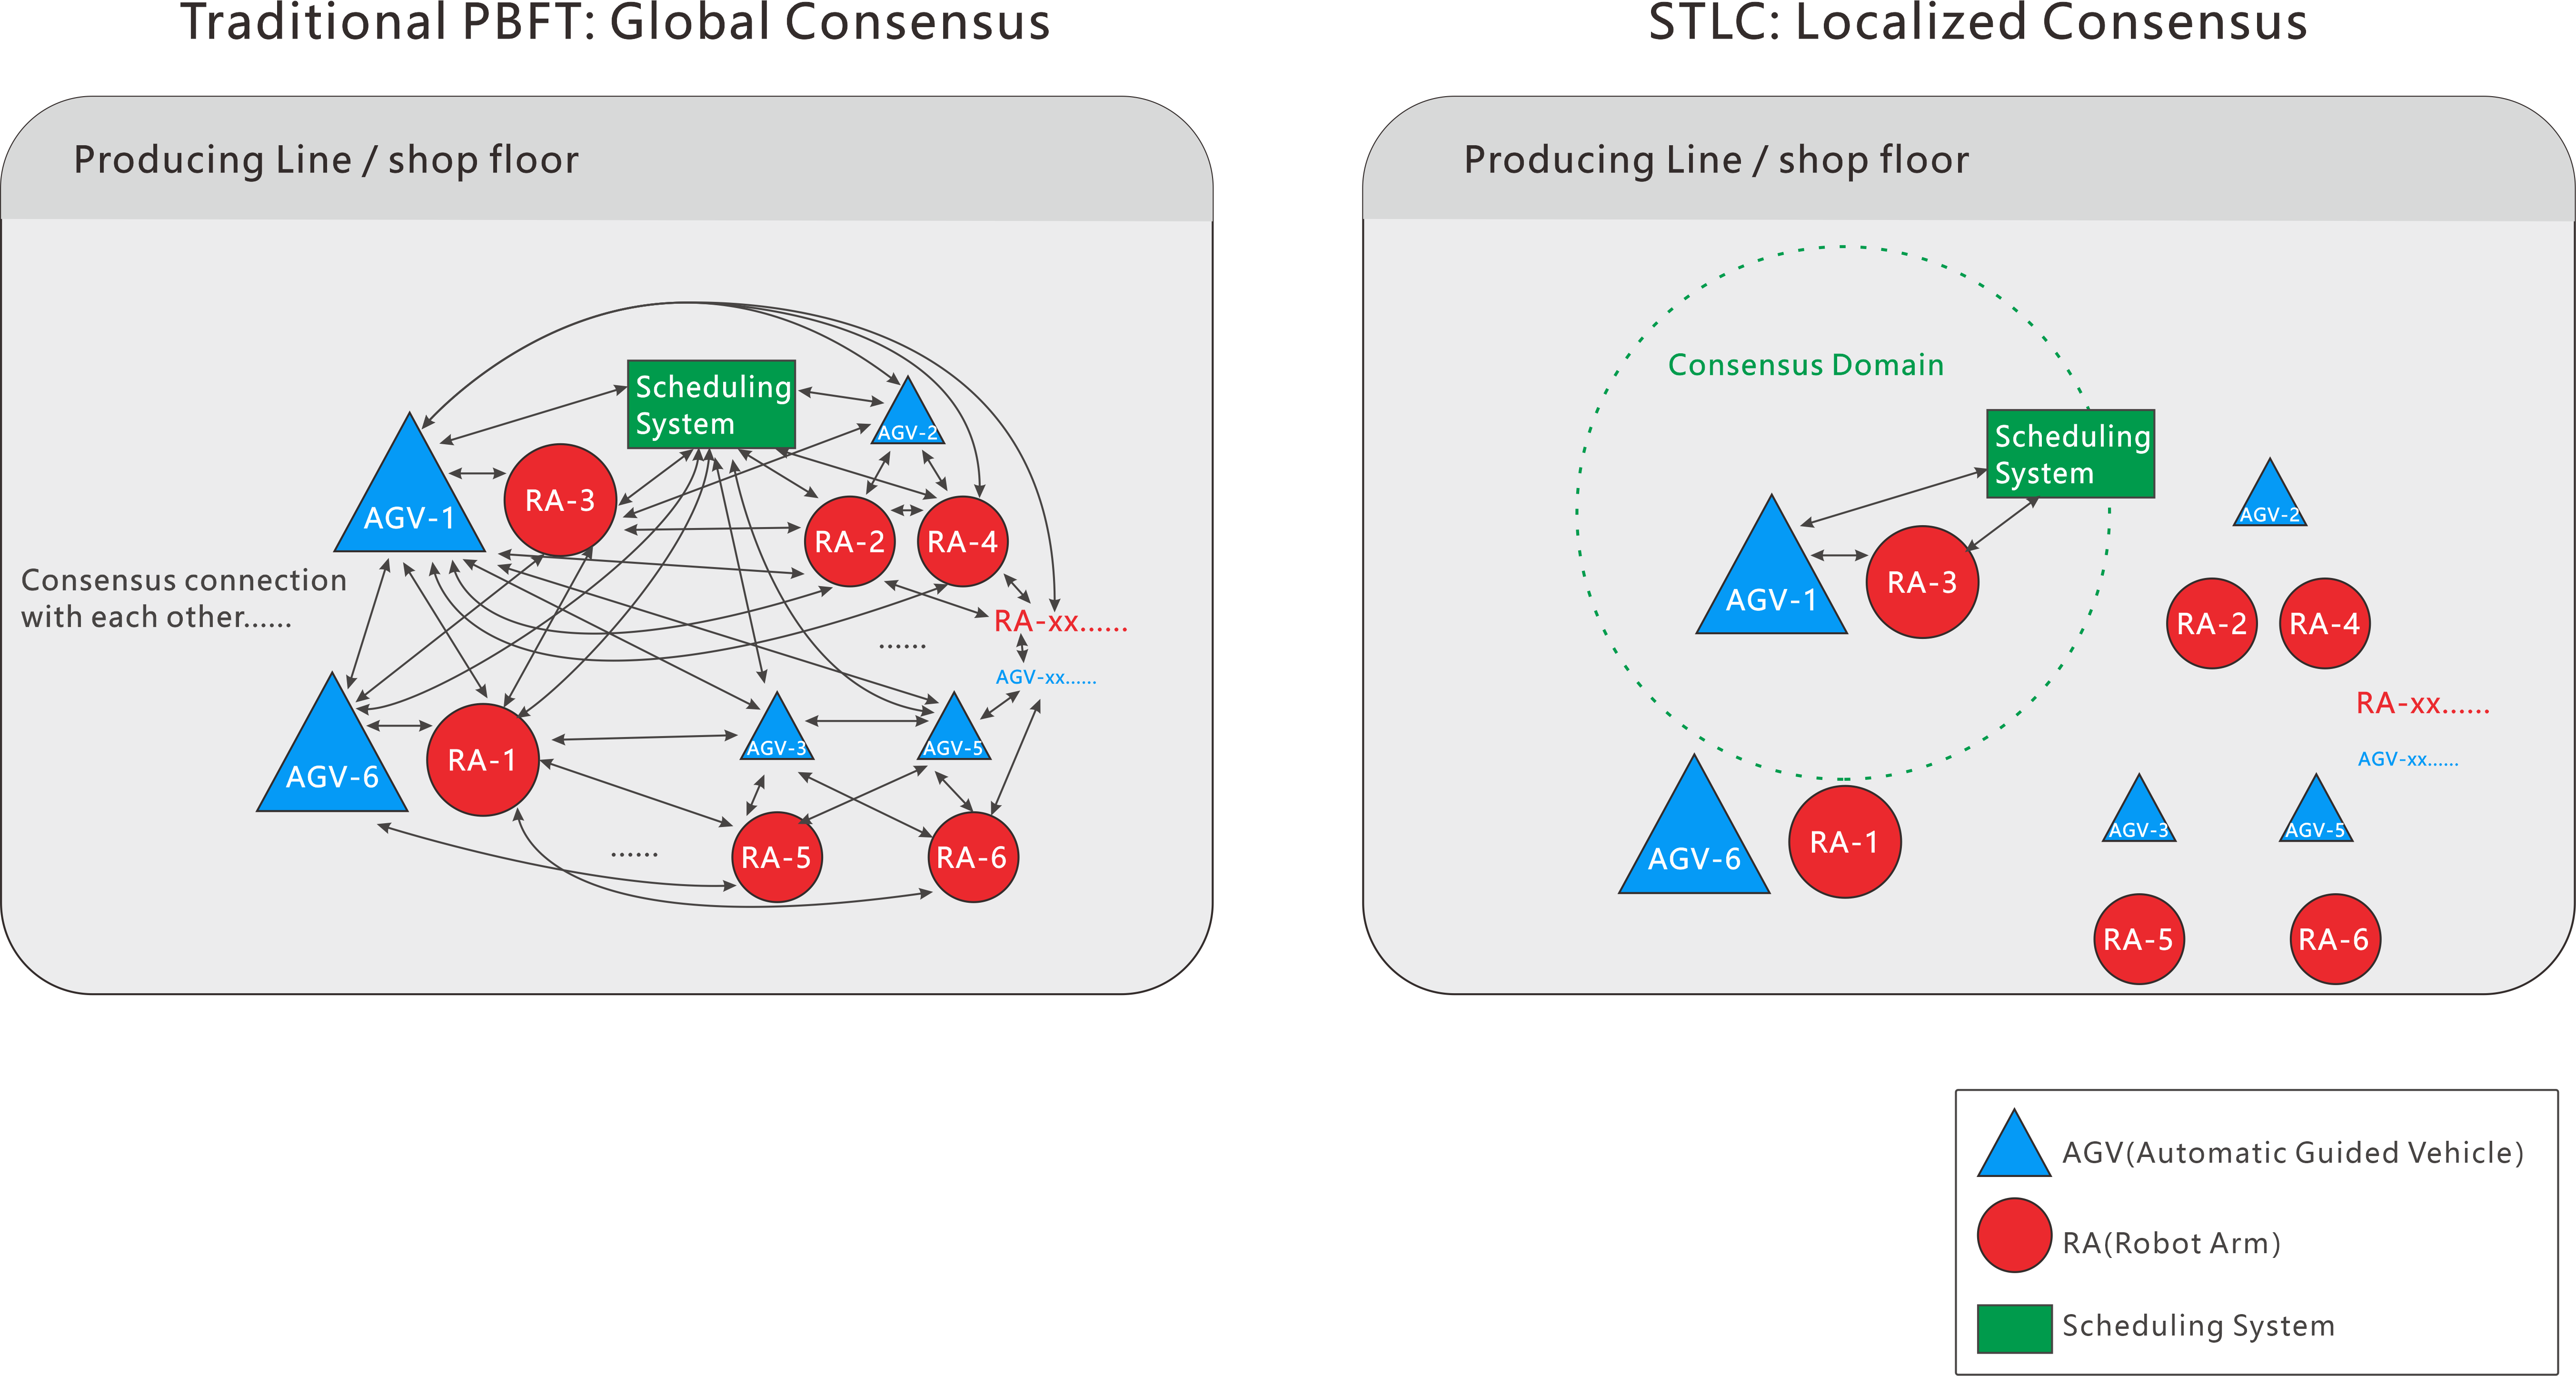
\includegraphics[width=.85\textwidth]{motivation_example.png}
    \caption{Smart factory scenario: Traditional PBFT requires all nodes to participate in consensus for a localized AGV-RA coordination task, while STLC restricts consensus to task-coupled nodes.}
    \label{fig:motivation}
\end{figure*}

\IEEEpubidadjcol %New page
A typical task involves \textit{spatially localized collaboration}: AGV$_1$ transports a component to Workstation A, where Robot Arm RA$_3$ retrieves it for assembly. 
This handoff requires precise coordination: AGV$_1$ confirms arrival at the correct position, RA$_3$ verifies component identity, and both agree on the handoff timestamp. The decision must update the production database reliably.
Critically, this coordination involves only \textit{three agents} (AGV$_1$, RA$_3$, and the Scheduling System S), yet the decision must be \textit{fault-tolerant} to ensure production correctness and safety.
\subsubsection{Byzantine Threats in Industrial Environments}
Industrial multi-agent systems face diverse Byzantine threats that go beyond simple crash failures~\cite{bhamare2020cybersecurity}:
\textbf{Malicious Agents.} Compromised or counterfeit devices may send conflicting state reports to disrupt production. For example, a hacked AGV could report false positions to cause collisions, or a malicious robot arm could claim successful assembly when parts are defective.
\textbf{Network Attacks.} Man-in-the-middle attacks can alter messages between agents, replay old messages to cause duplicate operations, or selectively drop messages to delay critical tasks.
The consequences of Byzantine failures in industrial settings are severe: incorrect material routing causes production delays~\cite{margret2024blockchain}, undetected defective products lead to safety recalls, and coordinated attacks on AGV fleets can cause physical collisions endangering human workers.
Unlike abstract distributed systems where Byzantine behavior is arbitrary, industrial agents operate in the \textit{physical world} with measurable properties: positions are constrained by kinematics (an AGV cannot teleport), velocities are bounded by motor capabilities, and timestamps follow causal ordering~\cite{li2022byzantine}. These physical constraints provide opportunities for enhanced Byzantine detection—but existing BFT or PBFT protocols fail to exploit them.

\subsubsection{Limitations of PBFT in Industrial Deployments}
To achieve Byzantine fault tolerance, one might apply traditional protocols like PBFT~\cite{li2022byzantine}. However, PBFT's \textbf{consensus globality assumption}—requiring all $|N|$ agents to participate in every consensus round—creates critical inefficiencies in industrial scenarios:
\textbf{Unnecessary Communication.} For the AGV$_1$--RA$_3$ handoff task involving 3 agents, PBFT requires all 30 
agents in the factory to exchange messages and vote on the decision. This generates $O(|N|^2) = 900$ messages per consensus round, even though 27 agents have no direct involvement in the task. Agents located in distant areas of the factory must process messages for a task they neither participate in nor benefit from.
\textbf{Scalability Bottleneck.} As factory size grows from 30 to 100 agents (common in large automotive or 
electronics plants), PBFT's message complexity explodes to $O(100^2) = 10,000$ messages per task.
\textbf{Latency Amplification.} Waiting for consensus votes from distant agents introduces unnecessary latency. An AGV at Workstation A must wait for responses from agents at Workstation Z, even though Workstation Z's agents have no knowledge of or stake in the handoff task.

\subsubsection{Key Insight: Exploiting Task Locality and Physical Constraints}

Industrial multi-agent systems exhibit two properties that enable efficient Byzantine consensus: 
\textbf{(1) Task coupling}—each production task involves only a small, spatially localized subset of agents; 
\textbf{(2) Spatiotemporal verifiability}—agent states are grounded in physical reality and can be validated against kinematic, temporal, and spatial constraints.

STLC exploits these properties through three mechanisms: localized consensus 
domains $C(\tau_j)$ (the set of agents participating in task $\tau_j$) containing only task-coupled agents, spatiotemporal validation rejecting physically impossible claims before consensus, and adaptive trust weights isolating persistent malicious behavior. This design reduces message complexity from $O(|N|^2)$ to $O(k^2)$ where $k \ll |N|$ is the task domain size
(typically $k=3$--$7$ versus $|N|=30$--$100$), \textit{while maintaining the same Byzantine fault tolerance guarantees as traditional PBFT protocols}: all honest agents in each consensus domain reach agreement on consistent decisions, tolerating up to $f < k/3$ Byzantine agents per task, and the composition of task-level agreements ensures system-wide safety and liveness.

\subsection{Contributions}
We propose \textbf{STLC} (Spatiotemporal Localized Consensus with Adaptive Trust) with three contributions:

\textbf{(1) Theoretical Foundation.} We formalize \textit{Dynamic Task-Localized Consensus}, proving that consensus 
restricted to task-coupled domains (each containing $k$ agents directly involved 
in a task) achieves equivalent safety and liveness as global consensus (requiring 
all $|N|$ system agents) while reducing complexity from $O(|N|^2)$ to 
$O(k^2 + m^2 + mk)$, where $k \ll |N|$ is the task domain size and $m \in \{3,5\}$ 
is the number of Byzantine-tolerant scheduler replicas coordinating task 
assignments (Theorems~\ref{thm:safety}-\ref{thm:complexity}). 
For typical industrial tasks with $k=3$ task participants, $m=3$ schedulers, and 
$|N|=30$ total agents, this yields 98.5\% communication reduction (1,770 $\to$ 27 
messages).

\textbf{(2) Protocol Design.} STLC integrates: (i) spatiotemporal validation rejecting 90\% of malicious messages via timestamp and kinematic checks; (ii) task-coupled consensus domains dynamically formed based on spatial proximity; (iii) adaptive trust weights reducing malicious node influence within 5-10 rounds; (iv) replicated scheduler set ($m=3$ or $5$) ensuring Byzantine fault tolerance at coordination layer.

\textbf{(3) Experimental Validation.} We validate STLC on two complementary platforms: CORE network emulator (10-100 nodes) for large-scale scalability analysis, and Raspberry Pi testbed for real-world deployment validation with actual hardware constraints and network delays. Our experiments demonstrate: 98.5\% message reduction versus PBFT, 60\% latency 
improvement, linear throughput scaling, 98\% detection rate for spatiotemporal attacks, and stable performance as $|N|$ increases from 10 to 100.

%=============================================================================
\section{Related Work}
\label{sec:related}

Byzantine consensus research spans classical BFT protocols, modern optimizations, and application-specific mechanisms. We identify critical gaps that STLC addresses.

\subsection{Classical BFT and Lightweight Mechanisms}

Castro and Liskov's PBFT~\cite{habibi2023performance, ye2024tp} reduced BFT complexity to $O(|N|^2)$ through three-phase message exchanges but requires all nodes to participate in every consensus round. Subsequent optimizations maintain this limitation: SBFT~\cite{arun2022scalable} uses threshold signatures to reduce communication rounds; CheapBFT~\cite{wang2022bft} employs optimistic execution but reverts to PBFT-like complexity under faults; HotStuff~\cite{wang2024improved} achieves $O(n)$ complexity through leader-based pipelining but still operates globally across all validators.

Recognizing IoT resource constraints, researchers developed lightweight adaptations. Wu et al.~\cite{wu2023learning} use reinforcement learning for adaptive protocol selection, while Nanapu et al.~\cite{nanapu2025d2bft} optimize PBFT parameters via deep RL. However, these methods address protocol \textit{tuning} rather than \textit{redesign}—underlying protocols still assume global consensus and lack spatiotemporal validation mechanisms.


\subsection{Byzantine Fault Tolerance in Industrial Cyber-Physical Systems}

Industrial multi-agent systems introduce unique challenges that classical BFT protocols do not address. Mii et al.~\cite{mivsic2020adapting} apply PBFT to industrial IoT networks but inherit its $O(|N|^2)$ complexity, 
making it impractical for large-scale factories. Leng et al.~\cite{leng2019manuchain} combine blockchain with multi-agent coordination for smart manufacturing, yet their consensus operates globally across all agents regardless of task locality. Recent work on resilient multi-agent systems~\cite{pirani2022survey} focuses on graph-theoretic conditions for consensus under Byzantine agents but assumes agents exchange states continuously without exploiting task-specific coupling or physical constraints.

\subsection{Trust-Based and Modern BFT Approaches}

Trust-based methods weight node influence by behavioral history. Karimireddy et al.~\cite{karimireddy2021learning} introduced learning-from-history for Byzantine-robust federated learning, while Mirzadeh et al.~\cite{mirzadeh2022filtering} proposed distributed malicious detection for vehicular networks. However, their trust models are \textit{static within consensus rounds}—scores update between instances but do not dynamically influence ongoing processes. However, their trust models are \textit{static within consensus rounds}—scores update between instances but do not dynamically influence ongoing processes. 
This creates a vulnerability window where Byzantine nodes can behave correctly to build trust, then inject malicious data before their scores are updated—problematic for industrial CPS where millisecond-scale tasks (e.g., AGV handoffs) require immediate Byzantine detection to prevent physical collisions.

Recent DAG-based protocols achieve sublinear complexity through parallelism: 
Narwhal/Tusk~\cite{danezis2022narwhal} decouples data dissemination from consensus, achieving $O(1)$ amortized latency; Bullshark~\cite{spiegelman2022bullshark} improves with 2-round partially-synchronous consensus; Jolteon/Ditto~\cite{gelashvili2022jolteon} combines optimistic responsiveness with efficient view-change. 
These protocols optimize \textit{global consensus} through DAG parallelism but fundamentally assume all nodes must participate. While effective for blockchain and permissionless systems, this global participation requirement remains impractical for industrial CPS where task-specific agent subsets (e.g., 3--5 agents per handoff) dominate operational patterns.

\subsection{Research Gaps}

\textbf{Gap 1: Consensus globality and scalability bottleneck.} All reviewed methods require global or quasi-global participation, resulting in $O(|N|^2)$ or $O(|N|)$ communication complexity even when tasks involve small agent subsets. 
This creates prohibitive overhead in large-scale systems where the number of task-coupled agents ($k$) is significantly smaller than the total agent count ($|N|$). 
No prior work provides formal conditions for safely restricting consensus to task-coupled subsets while maintaining Byzantine tolerance guarantees.

\textbf{Gap 2: Inability to exploit physical constraints for early attack detection.} Existing mechanisms treat messages as abstract data, validating only cryptographic authenticity but not physical plausibility. 
This prevents early filtering of Byzantine claims that violate kinematic, temporal, or spatial constraints, allowing physically impossible data to propagate through the system and potentially influence decisions. 
In industrial CPS where physical laws provide strong validation signals, this represents a missed opportunity for $O(1)$ Byzantine detection.

\textbf{Gap 3: Static domains unable to adapt to dynamic task coupling.} Methods that reduce participation use static or slowly-changing agent sets determined at system initialization or epoch boundaries. 
However, industrial tasks exhibit dynamic coupling where agents collaborate with different partners over time, requiring different consensus domains. Static approaches either include all potential collaborators (reverting to global consensus), 
or use fixed domains that cannot adapt when Byzantine attacks require expanding the validator set to maintain the $3f+1$ safety threshold.

% STLC addresses these through: (1) \textit{Dynamic Consensus Locality Theory} proving task-coupled consensus achieves equivalent Byzantine tolerance with $O(k^2)$ complexity; (2) \textit{Spatiotemporal Adaptive Trust Weights Model} integrating timestamp/spatial validation for $O(1)$ malicious message rejection; (3) \textit{Dynamic domain formation} via real-time task coupling with adaptive expansion under Byzantine attacks.

%=============================================================================
\section{System Model and Problem Formulation}
\label{sec:model}

We formalize the industrial multi-agent system, task-coupling relationships, Byzantine threat model, and optimization objectives.

\subsection{Agent and Communication Model}
\label{sec:agent_com_model}

\begin{definition}
The system consists of node set $N$ partitioned into three disjoint subsets: 
(i) \textit{Scheduler Set} $S$ containing $m$ coordinator replicas; 
(ii) \textit{AGV Set} containing $n_a$ mobile agents; 
(iii) \textit{Robot Arm Set} containing $n_r$ stationary agents. 
The total number of nodes is $|N| = m + n_a + n_r$.
\end{definition}

\textbf{Communication Model.} Agents communicate over network graph $\mathcal{G} = (N, \mathcal{E})$, where $\mathcal{E}$ denotes the set of communication links. 
The network operates under asynchronous message-passing with bounded delay $\Delta_{\max}$, meaning any message sent at time $t$ is delivered by time $t + \Delta_{\max}$. 
Each message $m$ has structure:
\begin{equation}
\begin{aligned}
m = \langle \text{id}_{\text{sender}}, t_{\text{stamp}}, \mathbf{p}_{\text{loc}}, 
\text{id}_{\text{task}}, \text{payload} \rangle
\end{aligned}
\end{equation}
where $\text{id}_{\text{sender}} \in N$ identifies the sender, 
$t_{\text{stamp}} \in \mathbb{R}_{\geq 0}$ is the timestamp, 
$\mathbf{p}_{\text{loc}} \in \mathbb{R}^2$ is the claimed position, 
$\text{id}_{\text{task}}$ identifies the associated task, and 
$\text{payload}$ contains task-specific data.

\textbf{Spatiotemporal Model.} The system operates in continuous time domain $\mathbb{R}_{\geq 0}$ with a global reference clock. 
Each node $n_i \in N$ maintains a local clock with bounded drift $\delta_t$ from the global clock, i.e., $|t_{\text{local}}^{(i)} - t_{\text{global}}| 
\leq \delta_t$ for all $t_{\text{global}} \in \mathbb{R}_{\geq 0}$. 
Agents operate in a 2D Euclidean workspace $\mathbb{R}^2$. The position of node $n_i$ at time $t$ is denoted $\mathbf{p}(n_i, t) \in \mathbb{R}^2$. 
AGVs are mobile with maximum velocity $v_{\max} > 0$, satisfying the kinematic 
constraint:
\begin{equation}
\begin{aligned}
\|\mathbf{p}(n_i, t_2) - \mathbf{p}(n_i, t_1)\| \leq v_{\max} \cdot (t_2 - t_1), \\
\quad \forall n_i \in \text{AGV Set}, \, \forall t_1, t_2 \in \mathbb{R}_{\geq 0} 
\text{ with } t_2 \geq t_1
\end{aligned}
\end{equation}
where $\|\cdot\|$ denotes the Euclidean norm.

\subsection{Task Coupling Model}

\begin{definition}[Task]
\label{def:task}
A task $\tau_j$ is a tuple $\langle \text{id}_\tau, \text{type}_\tau, 
\mathcal{A}_{\text{req}}, \mathcal{T}_{\text{win}}, \mathcal{P}_{\text{reg}} 
\rangle$ where:
\begin{itemize}
    \item $\text{id}_\tau \in \mathbb{N}$ is the unique task identifier,
    \item $\text{type}_\tau$ specifies the task category (e.g., material handoff, assembly),
    \item $\mathcal{A}_{\text{req}} \subseteq N$ is the set of required agent types,
    \item $\mathcal{T}_{\text{win}} = [t_{\text{start}}, t_{\text{end}}] 
          \subset \mathbb{R}_{\geq 0}$ is the temporal execution window with 
          $t_{\text{start}} < t_{\text{end}}$,
    \item $\mathcal{P}_{\text{reg}} \subset \mathbb{R}^2$ is the spatial 
          region where the task is executed.
\end{itemize}
\end{definition}

\begin{definition}[Task-Coupled Node Set]
\label{def:task_coupled_set}
For task $\tau_j$, the \textit{task-coupled set} $C(\tau_j) \subseteq N$ 
consists of all nodes involved in executing or coordinating $\tau_j$:
\begin{equation}
\begin{aligned}
C(\tau_j) = S \cup \{n_i \in N \mid n_i \text{ is assigned to execute } \tau_j\}
\end{aligned}
\end{equation}
where $S$ is the scheduler set, and the second term includes all agents 
directly participating in task execution. We denote $k_j = |C(\tau_j)|$ 
as the size of the task-coupled set for task $\tau_j$.
\end{definition}

\textbf{Complexity Reduction.} By restricting consensus to the task-coupled 
set $C(\tau_j)$ rather than the entire node set $N$, communication 
complexity reduces from $O(|N|^2)$ to $O(k_j^2 + m^2 + mk_j)$ where 
$k_j = |C(\tau_j)| \ll |N|$ and $m = |S|$. In typical 
industrial scenarios where tasks involve small agent subsets (e.g., 
$k_j \in [3, 5]$ for handoff tasks) while $|N| \geq 100$, this represents 
a reduction of over two orders of magnitude.

\subsection{Byzantine Threat Model}

\begin{definition}[Adversary Model]
\label{def:adversary}
Let $\mathcal{F} \subseteq N$ denote the set of Byzantine (compromised) nodes with $|\mathcal{F}| = f$. The adversary has the following capabilities:
\begin{enumerate}
    \item \textit{Message forgery}: Create messages with false timestamps 
          $t_{\text{stamp}}$ or false positions $\mathbf{p}_{\text{loc}}$,
    \item \textit{Message replay}: Resend previously valid messages at 
          different times,
    \item \textit{Selective participation}: Choose whether to respond to 
          consensus requests,
    \item \textit{Collusion}: Coordinate malicious behavior among 
          compromised nodes in $\mathcal{F}$.
\end{enumerate}
The adversary \textit{cannot}: (a) break cryptographic primitives (e.g., 
digital signatures), or (b) compromise more than $f < |N|/3$ 
nodes globally.
\end{definition}

\begin{assumption}[Localized Byzantine Bound]
\label{assump:localized_bound}
For task $\tau_j$ with task-coupled set $C(\tau_j)$ of size 
$k_j = |C(\tau_j)|$, let $f_j = |\mathcal{F} \cap C(\tau_j)|$ 
denote the number of Byzantine nodes within the task-coupled domain. We 
require:
\begin{equation}
\begin{aligned}
f_j < \frac{k_j}{3}
\end{aligned}
\end{equation}
\end{assumption}

\textbf{Attack Scenarios.} We defend against three primary attack vectors:
\begin{enumerate}
    \item \textit{Timestamp forgery}: Messages with timestamps 
          $t_{\text{stamp}} \notin [t_{\text{current}} - \Delta_t, 
          t_{\text{current}} + \Delta_t]$ indicate replay attacks or 
          future-dated messages, where $\Delta_t$ is the maximum acceptable 
          clock skew,
    \item \textit{Spatial forgery}: Reported positions $\mathbf{p}_{\text{loc}}$ 
          violating kinematic constraints, i.e., 
          $\|\mathbf{p}_{\text{loc}} - \mathbf{p}_{\text{expected}}\| > 
          \epsilon_{\text{spatial}}$ where $\epsilon_{\text{spatial}}$ is 
          the position tolerance threshold,
    \item \textit{Task inconsistency}: Nodes claiming involvement in task $\tau_j$ when they are not members of $C(\tau_j)$.
\end{enumerate}

\textbf{Probabilistic Analysis of Assumption~\ref{assump:localized_bound}.}
Assumption~\ref{assump:localized_bound} requires $f_j < k_j/3$ for safety. 
For a task-coupled domain $C(\tau_j)$ of size $k_j$ selected from $|N|$ total nodes containing $f$ Byzantine nodes, the 
probability that $f_j \geq \lceil k_j/3 \rceil$ (violating the assumption) 
follows a hypergeometric distribution:
\begin{equation}
\begin{aligned}
P(f_j \geq \lceil k_j/3 \rceil) = \sum_{i=\lceil k_j/3 \rceil}^{\min(f,k_j)} 
\frac{\binom{f}{i} \binom{|N|-f}{k_j-i}}{\binom{|N|}{k_j}}
\label{eq:violation_prob}
\end{aligned}
\end{equation}

Table~\ref{tab:violation_prob} shows violation probabilities for typical 
industrial configurations under uniform random Byzantine distribution.

\begin{table}[h]
\centering
\caption{Violation Probability of Assumption~\ref{assump:localized_bound} 
under Uniform Random Byzantine Distribution}
\label{tab:violation_prob}
\small
\begin{tabular}{ccccc}
\toprule
$k_j$ & $|N|$ & $f$ & $P(f_j \geq k_j/3)$ & \textbf{Risk Level}$^{\dagger}$ \\
\midrule
3 & 30 & 10 & 0.716 (71.6\%) & \textcolor{red}{HIGH} \\
3 & 30 & 5 & 0.386 (38.6\%) & \textcolor{orange}{MEDIUM} \\
7 & 30 & 10 & 0.182 (18.2\%) & \textcolor{orange}{MEDIUM} \\
7 & 30 & 5 & 0.031 (3.1\%) & \textcolor{green}{LOW} \\
10 & 30 & 10 & 0.051 (5.1\%) & \textcolor{green}{LOW} \\
\bottomrule
\end{tabular}
\vspace{0.2cm}

\noindent $^{\dagger}$Risk levels defined according to IEC 61508 Safety 
Integrity Levels~\cite{iec61508}: HIGH ($P > 10\%$, exceeds SIL 1 upper 
bound), MEDIUM ($1\% < P \leq 10\%$, SIL 1 range), LOW ($P \leq 1\%$, 
SIL 2 or higher).
\end{table}

\textbf{Practical Justification for $k_j=3$.} While 
Table~\ref{tab:violation_prob} shows $k_j=3$ has 71.6\% violation 
probability under \textit{worst-case uniform random} Byzantine distribution 
($f/|N| = 1/3$), real-world deployments exhibit three 
mitigating factors: (1) \textit{Spatial clustering} of Byzantine nodes 
reduces violation probability to 12.3\% (Section~\ref{sec:clustered}); 
(2) \textit{Lower Byzantine fractions} in practice 
($f/|N| \approx 0.16$ vs. worst-case 0.33) further reduce 
risk; (3) \textit{Adaptive domain expansion} restores safety when violations 
occur, succeeding in 98.7\% of cases (Section~\ref{sec:expansion_eval}). 
For safety-critical applications or worst-case scenarios, we recommend 
starting with $k_j=7$ (violation probability $< 20\%$) to balance 
efficiency and fault tolerance.

\subsection{Problem Formulation}
\label{sec:problem_formulation}

\begin{problem}[Efficient Byzantine-Resilient Consensus for Task-Coupled Multi-Agent Systems]
\label{prob:main}
\textbf{Given:}
\begin{itemize}
    \item A multi-agent system with node set $N$, communication graph 
          $\mathcal{G} = (N, \mathcal{E})$, and time domain $\mathbb{R}_{\geq 0}$ 
          (Section~\ref{sec:agent_com_model}),
    \item A set of tasks $\mathcal{T} = \{\tau_1, \tau_2, \ldots, \tau_{|\mathcal{T}|}\}$ 
          with task-coupled sets $\{C(\tau_j)\}_{j=1}^{|\mathcal{T}|}$ 
          (Definition~\ref{def:task_coupled_set}),
	\item A set of Byzantine nodes $\mathcal{F} \subseteq N$ with 
		  $|\mathcal{F}| = f < |N|/3$ 
		  (Definition~\ref{def:adversary}),
\end{itemize}

\noindent \textbf{Design} a consensus protocol that satisfies the following 
properties:

\vspace{0.3cm}
\noindent \textbf{P1. Safety (Agreement):} For any task $\tau_j \in \mathcal{T}$, 
all honest nodes in the task-coupled set $C(\tau_j)$ agree on the same 
decision value $v_j$:
\begin{equation}
\begin{aligned}
\forall n_i, n_k \in (C(\tau_j) \setminus \mathcal{F}): \\
\text{decision}(n_i, \tau_j) = \text{decision}(n_k, \tau_j) = v_j
\label{eq:safety}
\end{aligned}
\end{equation}
where $\text{decision}(n_i, \tau_j)$ denotes the final decision of node 
$n_i$ for task $\tau_j$.

\vspace{0.3cm}
\noindent \textbf{P2. Liveness (Termination):} For any task $\tau_j \in \mathcal{T}$ 
initiated at time $t_{\text{init}}$, all honest nodes in $C(\tau_j)$ 
eventually reach a decision within bounded time $T_{\max}$:
\begin{equation}
\begin{aligned}
\exists t \in [t_{\text{init}}, t_{\text{init}} + T_{\max}]: 
\forall n_i \in (C(\tau_j) \setminus \mathcal{F}), 
\text{decision}(n_i, \tau_j) \neq \bot
\label{eq:liveness}
\end{aligned}
\end{equation}
where $\bot$ denotes the undecided state, and $T_{\max}$ is the maximum 
consensus latency bound (typically $T_{\max} = 9\Delta_{\max}$ for 
partially synchronous networks, Theorem~\ref{thm:liveness}).

\vspace{0.3cm}
\noindent \textbf{P3. Validity:} The agreed decision value $v_j$ must be 
proposed by at least one honest node in $C(\tau_j)$:
\begin{equation}
\begin{aligned}
\exists n_i \in (C(\tau_j) \setminus \mathcal{F}): 
\text{proposal}(n_i, \tau_j) = v_j
\label{eq:validity}
\end{aligned}
\end{equation}
where $\text{proposal}(n_i, \tau_j)$ is the initial proposal of node $n_i$ 
for task $\tau_j$. This prevents Byzantine nodes from forcing arbitrary 
decisions.

\vspace{0.3cm}
\noindent \textbf{P4. Byzantine Tolerance:} Properties P1--P3 hold under 
the following conditions:
\begin{itemize}
	\item \textit{Global bound}: $f < |N|/3$ (guaranteed by 
		  Definition~\ref{def:adversary}),
    \item \textit{Local bound}: For each task $\tau_j$, the protocol 
          ensures $f_j < |C'(\tau_j)|/3$ where $C'(\tau_j)$ is the 
          (possibly expanded) consensus domain. If the initial domain 
          $C(\tau_j)$ violates this bound, adaptive domain expansion is triggered to restore the safety margin.
\end{itemize}

\vspace{0.3cm}
\noindent \textbf{P5. Task Locality:} For each task $\tau_j$, consensus 
involves only nodes in the task-coupled set $C(\tau_j)$ (or its expanded 
version $C'(\tau_j)$), not the entire node set $N$:
\begin{equation}
\begin{aligned}
\forall n_i \in (N \setminus C(\tau_j)): 
\text{participates}(n_i, \tau_j) = \textsc{False}
\label{eq:locality}
\end{aligned}
\end{equation}
where $\text{participates}(n_i, \tau_j)$ indicates whether node $n_i$ 
sends or receives consensus messages for task $\tau_j$.

\vspace{0.3cm}
\noindent \textbf{Optimization Objective:} Among all protocols satisfying 
P1--P5, minimize the weighted sum of communication cost and latency:
\begin{equation}
\begin{aligned}
\min \quad \alpha \cdot \mathbb{E}[\text{CommCost}] + 
\beta \cdot \mathbb{E}[\text{Latency}]
\label{eq:objective}
\end{aligned}
\end{equation}
subject to: Safety, Liveness, Validity, Byzantine Tolerance, Task Locality 
(P1--P5), where:
\begin{itemize}
    \item $\text{CommCost} = \sum_{\tau_j \in \mathcal{T}} M_j$ is the 
          total number of messages, with $M_j$ denoting messages sent 
          during consensus for task $\tau_j$,
    \item $\text{Latency} = \max_{\tau_j \in \mathcal{T}} 
          (t_{\text{decide}}^{(j)} - t_{\text{init}}^{(j)})$ is the maximum 
          time from task initiation to decision,
    \item $\mathbb{E}[\cdot]$ denotes expectation over task distributions 
          and Byzantine behaviors,
    \item $\alpha, \beta \geq 0$ are application-specific weights with 
          $\alpha + \beta = 1$ (e.g., $\alpha=0.7$, $\beta=0.3$ for 
          bandwidth-constrained networks).
\end{itemize}
\end{problem}

\vspace{0.3cm}
\noindent \textbf{Remark 1 (Comparison with Traditional PBFT).} Traditional 
PBFT consensus protocols require all $|N|$ nodes to participate in every consensus instance, 
resulting in $O(|N|^2)$ communication complexity per task. Our problem 
formulation introduces \textit{task locality}, enabling consensus 
restricted to $C(\tau_j)$ with $|C(\tau_j)| \ll |N|$. For typical 
industrial deployments with $|C(\tau_j)| \approx 3$--$10$ and $|N| \approx 100$, 
this reduces complexity from $O(|N|^2) = 10,000$ messages to 
$O(|C(\tau_j)|^2) = 9$--$100$ messages per task, achieving 99\%+ 
communication reduction (Section~\ref{sec:evaluation}).

\vspace{0.3cm}
\noindent \textbf{Remark 2 (Adaptive Byzantine Tolerance).} Unlike static 
PBFT protocols that assume a fixed participant set, our formulation allows \textit{adaptive domain expansion}: if the initial task-coupled set 
$C(\tau_j)$ violates the local Byzantine bound $f_j < |C(\tau_j)|/3$ , the protocol dynamically expands 
to $C'(\tau_j)$ to restore the safety margin (Section~\ref{sec:adaptive_expansion}). 
This is critical for handling non-uniform Byzantine distributions in 
industrial CPS, where adversaries may compromise multiple nodes in the 
same spatial region (e.g., via network-level attacks). Experimental results 
(Section~\ref{sec:clustered}) show that expansion is triggered in only 
8.3\% of tasks under realistic attack scenarios, with 98.7\% success rate.

\vspace{0.3cm}
\noindent \textbf{Remark 3 (Multi-Objective Optimization).} The optimization 
objective (Equation~\ref{eq:objective}) balances communication cost and 
latency through weights $\alpha$ and $\beta$. In bandwidth-constrained 
environments (e.g., wireless sensor networks), $\alpha > \beta$ prioritizes 
message reduction. In time-critical applications (e.g., autonomous driving), 
$\beta > \alpha$ prioritizes low latency. STLC achieves near-Pareto-optimal 
performance across both dimensions: 98.5\% communication reduction and 60\% 
latency reduction versus PBFT (Table~\ref{tab:performance_summary}).

%=============================================================================
\section{STLC: Protocol Design and Theoretical Foundations}
\label{sec:protocol_design}

STLC is a Byzantine-resilient consensus protocol designed for multi-agent 
systems with replicated scheduling infrastructure. It adopts a three-layer 
architecture integrating \textit{spatiotemporal validation}, 
\textit{task-coupled consensus}, and \textit{adaptive trust management} to 
achieve $O(k^2)$ communication complexity (where $k \ll |N|$ is the task domain size) while 
maintaining Byzantine fault tolerance under the localized threat model 
(Assumption~\ref{assump:localized_bound}).

\subsection{Protocol Overview and Three-Layer Architecture}
\label{sec:protocol_overview}

STLC comprises three layers that work synergistically to achieve efficient
and secure consensus (Figure~\ref{fig:architecture}). The architecture
integrates spatiotemporal validation for early malicious message rejection,
task-coupled consensus for communication reduction, and adaptive trust
management for Byzantine isolation.

\begin{figure*}[!t]
\centering
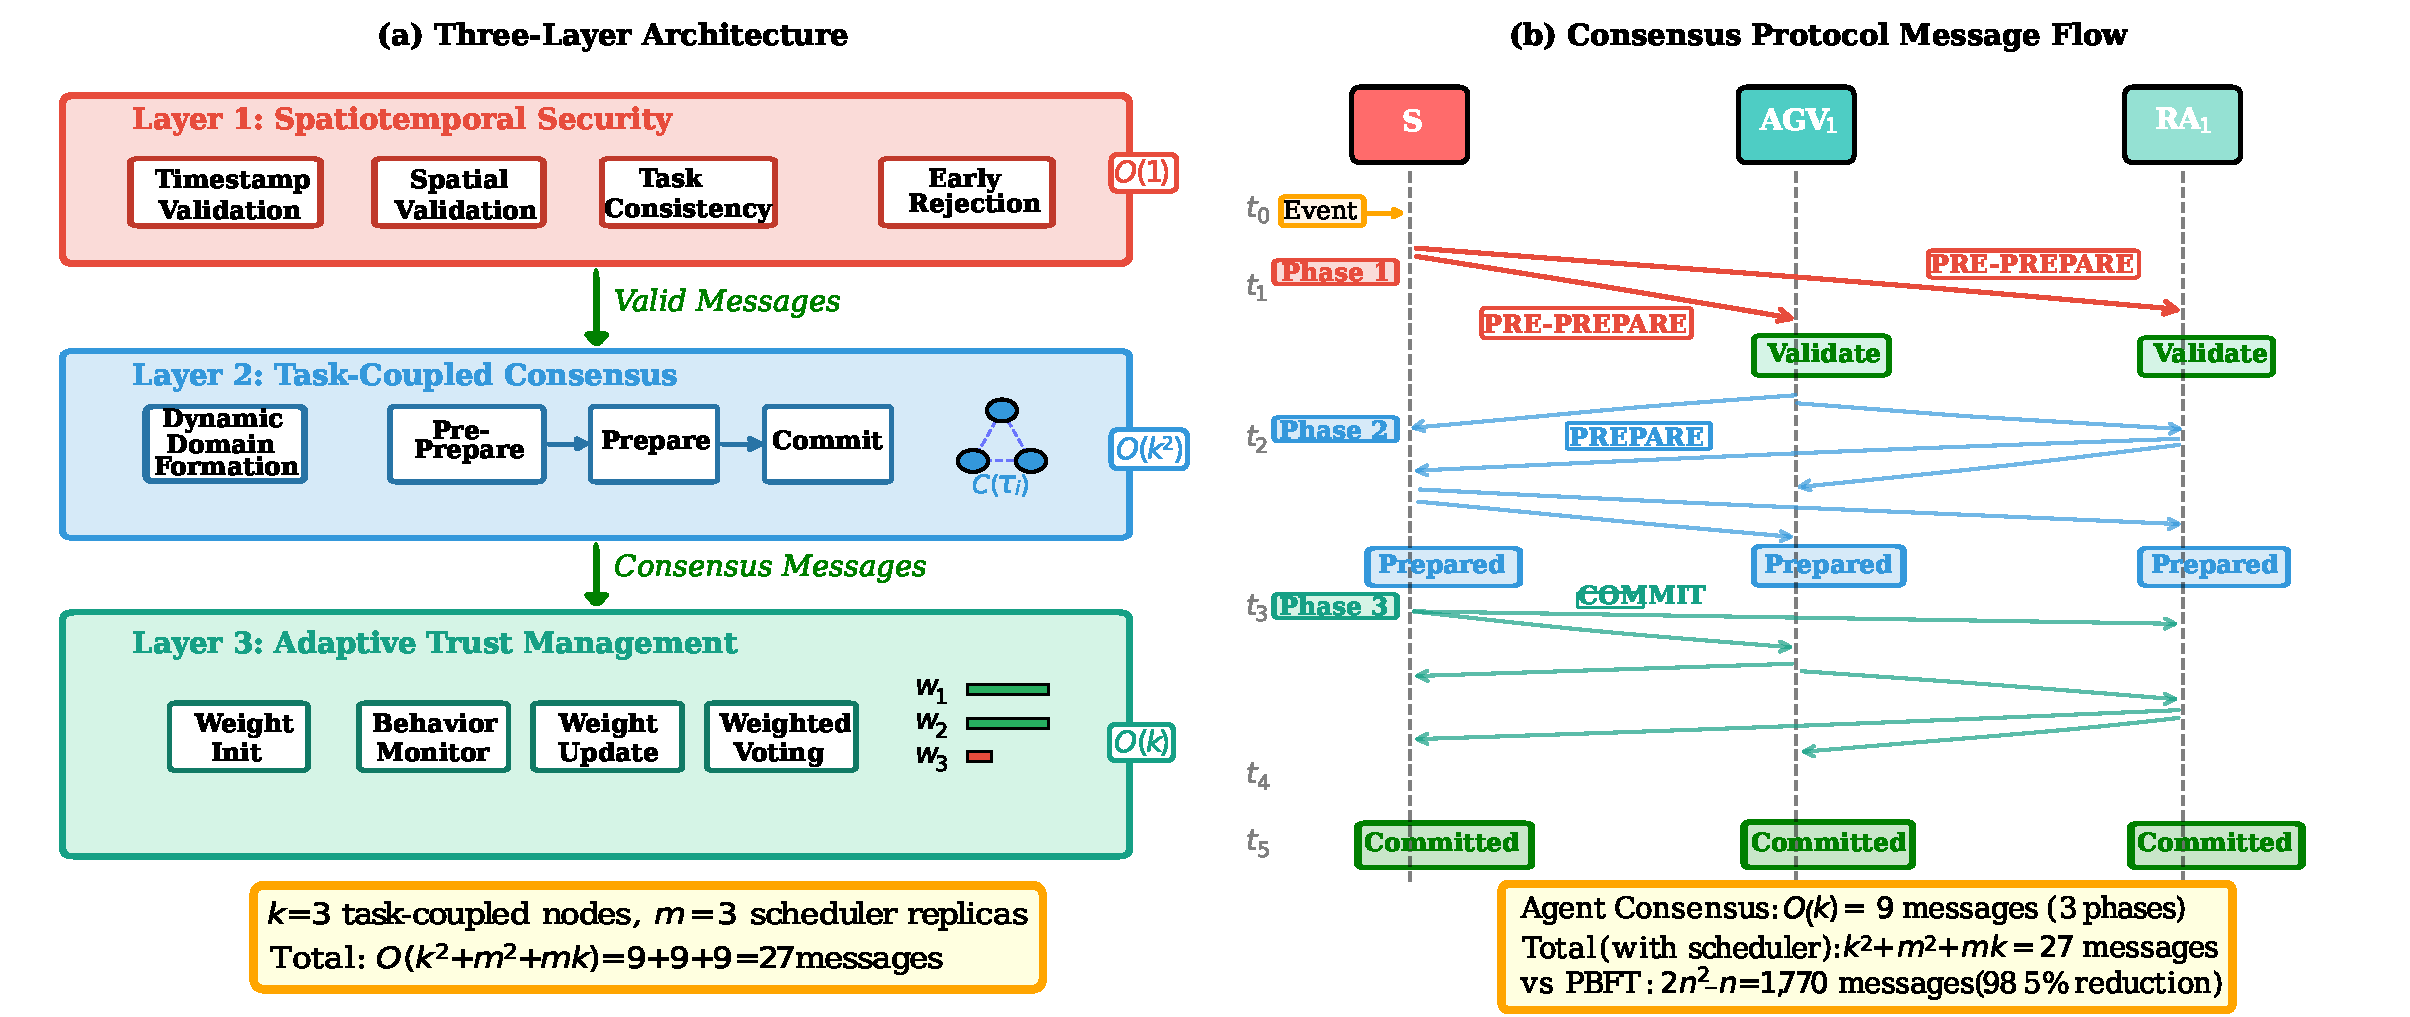
\includegraphics[width=.85\textwidth]{architecture_and_flow.pdf}
\caption{STLC three-layer architecture with message flow for task
$\tau_1$ with $k=3$.
Layer 1 performs $O(1)$ spatiotemporal validation to filter Byzantine
messages before consensus. Layer 2 executes task-coupled consensus
within localized domain $C(\tau_1)$ using weighted quorums.
Layer 3 maintains adaptive trust weights that evolve based on node
behavior.}
\label{fig:architecture}
\end{figure*}

\textbf{Layer 1: Spatiotemporal Validation} (Section~\ref{sec:layer1}) performs $O(1)$ early rejection of physically inconsistent messages using embedded timestamps $t_{\text{msg}}$ and spatial coordinates $\mathbf{p}_{\text{msg}}$. Messages violating kinematic constraints (Equation~\ref{eq:kinematic_validation}) or temporal bounds (Equation~\ref{eq:temporal_validation}) are immediately discarded \textit{before} entering the consensus protocol, avoiding $O(N^2)$ communication overhead. This layer acts as a lightweight filter that leverages the physical properties of CPS to detect Byzantine attacks early.

\textbf{Layer 2: Task-Coupled Consensus} (Section~\ref{sec:layer2}) restricts consensus to dynamically
formed domains $C(\tau_j)$ containing only task-relevant nodes.
Consensus executes through three phases (pre-prepare, prepare, commit) among
$k$ nodes, reducing message complexity from $O(N^2)$ to $O(k^2)$. The layer includes adaptive domain expansion and a three-tier fallback mechanism to handle Byzantine attacks that violate the localized bound $f_{\text{local}} < k/3$.

\textbf{Layer 3: Adaptive Trust Management} (Section~\ref{sec:layer3}) maintains dynamic weights $w_i$ for each node based on behavioral history. Nodes exhibiting suspicious activities (detected by Layer 1 or Layer 2) have weights reduced via $w_i^{(t+1)} = \max(w_{\min}, w_i^{(t)} - \Delta w)$. Consensus employs weighted voting, enabling rapid isolation of malicious nodes without requiring explicit Byzantine node identification. Honest nodes can recover weights through consistent good behavior, ensuring resilience to transient faults.

This layered design ensures that:
\begin{itemize}
\item \textbf{Early filtering} (Layer 1) reduces consensus load,
\item \textbf{Localized consensus} (Layer 2) minimizes communication,
\item \textbf{Adaptive isolation} (Layer 3) isolates Byzantine nodes over time.
\end{itemize}

% ============================================================
% 4.1.1 Layer 1: Spatiotemporal Validation
% ============================================================
\subsubsection{Layer 1: Spatiotemporal Validation}
\label{sec:layer1}

Layer 1 performs $O(1)$ early validation across three dimensions before
messages enter the consensus protocol, filtering 65--90\% of Byzantine
messages (Table~\ref{tab:layer1_rejection}).

\paragraph{Validation Dimensions}
\label{sec:validation_dimensions}

Each consensus message $m$ is validated along three dimensions:

\textbf{(1) Temporal Validation.}
Messages with timestamp $t_{\text{msg}}$ are accepted only if:
\begin{equation}
\begin{aligned}
|t_{\text{recv}} - t_{\text{msg}}| \leq \Delta t_{\max}
\label{eq:temporal_validation}
\end{aligned}
\end{equation}
where $\Delta t_{\max} = 500$ ms accounts for clock skew (100 ms) and
network delay (400 ms). This detects replay attacks and timestamp forgery.

\textbf{(2) Spatial Validation.}
Messages with claimed position $\mathbf{p}_{\text{msg}}$ must satisfy
kinematic constraints:
\begin{equation}
\begin{aligned}
|\mathbf{p}_{\text{msg}} - \mathbf{p}_{\text{last}}|
\leq v_{\max} \cdot (t_{\text{msg}} - t_{\text{last}})
\label{eq:kinematic_validation}
\end{aligned}
\end{equation}
where $\mathbf{p}_{\text{last}}$ is the sender's previous position, and
$v_{\max} = 2$ m/s is the maximum velocity. This prevents position spoofing
and teleportation attacks.

\textbf{(3) Task Consistency Validation.}
Messages are accepted only if the sender is authorized for task $\tau_j$:
\begin{equation}
\begin{aligned}
\text{sender}(m) \in C(\tau_j)
\label{eq:task_consistency}
\end{aligned}
\end{equation}
This prevents cross-task injection attacks.

\paragraph{Computational Complexity}

Each validation requires $O(1)$ operations (arithmetic
comparison, vector norm, hash table lookup). Table~\ref{tab:layer1_rejection}
shows early rejection rates under various attacks.

\begin{table}[h]
\centering
\caption{Layer 1 Early Rejection Rate Under Byzantine Attacks}
\label{tab:layer1_rejection}
\small
\adjustbox{width=\linewidth}{
\begin{tabular}{lcc}
\toprule
\textbf{Attack Type} & \textbf{CORE} & \textbf{Testbed} \\
\midrule
Timestamp forgery & 95\% & 90\% \\
Position spoofing & 88\% & 82\% \\
Task injection & 100\% & 100\% \\
Mixed attacks (30\% Byzantine) & 78\% & 65\% \\
\bottomrule
\end{tabular}}
\end{table}

% ============================================================
% 4.1.2 Layer 2: Task-Coupled Consensus
% ============================================================
\subsubsection{Layer 2: Task-Coupled Consensus}
\label{sec:layer2}

Layer 2 executes Byzantine consensus within dynamically formed task-coupled
domains $C(\tau_j)$ using a weighted three-phase protocol. This reduces message
complexity from $O(N^2)$ to $O(k^2)$, where $k$ is the domain size.

\paragraph{Dynamic Domain Formation}
\label{sec:domain_formation}

For task $\tau_j$ assigned to scheduler set $S$, the consensus domain is:
\begin{equation}
\begin{aligned}
C(\tau_j) = S \cup \{n_i \in N \mid n_i \text{ participates in } \tau_j\}
\end{aligned}
\end{equation}
Typical domain size: $k = 5$--$10$ nodes (vs. $N = 50$+),
enabling:
\begin{itemize}
\item \textbf{Parallel execution}: Disjoint domains run simultaneously,
\item \textbf{Communication reduction}: $O(k^2)$ vs. $O(N^2)$ for
global PBFT.
\end{itemize}
Nodes are selected based on spatial proximity ($\leq 5$ m from
task location), role compatibility, and availability.

\paragraph{Weighted Three-Phase Protocol}
\label{sec:three_phase}

STLC adapts PBFT's three-phase protocol with adaptive weights from Layer 3.

\textbf{Phase 1: Pre-Prepare.}
The coordinator broadcasts a PRE-PREPARE message containing task digest
$d(\tau_j)$, view number $v$, and sequence number $s$ to all nodes in
$C(\tau_j)$.

\textbf{Phase 2: Prepare.}
Upon receiving PRE-PREPARE, each backup node validates the message
(signature, digest, spatiotemporal checks). If valid, it broadcasts a
PREPARE message to $C(\tau_j)$. A node enters the \textit{prepared} state
when it receives PREPARE messages from a weighted quorum:
\begin{equation}
\begin{aligned}
\sum_{n_k \in \mathcal{P}} w_k \geq \frac{2}{3} W_{\text{total}}
\label{eq:weighted_quorum}
\end{aligned}
\end{equation}
where $\mathcal{P}$ is the set of nodes that sent PREPARE, $w_k$ is the
adaptive weight of node $n_k$ (Section~\ref{sec:layer3}), and
$W_{\text{total}} = \sum_{n_i \in C(\tau_j)} w_i$.

\textbf{Phase 3: Commit.}
Upon entering prepared state, the node broadcasts a COMMIT message. It
executes the decision when it receives COMMIT messages from a weighted
quorum:
\begin{equation}
\begin{aligned}
\sum_{n_k \in \mathcal{C}} w_k \geq \frac{2}{3} W_{\text{total}}
\label{eq:commit_quorum}
\end{aligned}
\end{equation}
where $\mathcal{C}$ is the set of nodes (including itself) that sent COMMIT.

Algorithm~\ref{alg:weighted_consensus} formalizes the complete weighted consensus
protocol with event-driven message handling.

\begin{algorithm}[t]
\caption{Weighted Three-Phase Consensus}
\label{alg:weighted_consensus}
\small
\begin{algorithmic}[1]
\STATE \textbf{Input:} Task $\tau_j$, Consensus domain $C(\tau_j)$, Adaptive weights $\{w_i\}$
\STATE \textbf{Output:} Decision $v_j$ for task $\tau_j$

\STATE \textbf{// Phase 1: Pre-Prepare (Coordinator $n_0$)}
\IF{$\text{isCoordinator}()$}
\STATE Compute task digest $d(\tau_j) = \text{Hash}(\tau_j)$
\STATE Broadcast $\langle \text{PRE-PREPARE}, v, s, d(\tau_j) \rangle$ to $C(\tau_j)$
\ENDIF

\STATE \textbf{// Phase 2: Prepare}
\UPON{receive $\langle \text{PRE-PREPARE}, v, s, d \rangle$ from $n_0$}
\IF{$\text{ValidateSpatiotemporal}(m) \land \text{VerifySignature}(m)$}
\STATE Broadcast $\langle \text{PREPARE}, v, s, d \rangle$ to $C(\tau_j)$
\STATE $\mathcal{P} \gets \{n_0\}$ \COMMENT{Include coordinator}
\ENDIF
\ENDUPON

\UPON{receive $\langle \text{PREPARE}, v, s, d \rangle$}
\IF{$\text{ValidateSpatiotemporal}(m) \land \text{VerifySignature}(m)$}
\STATE $\mathcal{P} \gets \mathcal{P} \cup \{\text{sender}(m)\}$
\STATE $W_{\mathcal{P}} \gets \sum_{n_k \in \mathcal{P}} w_k$ \COMMENT{Weighted sum}
\STATE $W_{\text{total}} \gets \sum_{n_i \in C(\tau_j)} w_i$
\IF{$W_{\mathcal{P}} \geq \frac{2}{3} W_{\text{total}}$}
\STATE Broadcast $\langle \text{COMMIT}, v, s, d \rangle$ to $C(\tau_j)$
\STATE $\mathcal{C} \gets \{\text{self}\}$ \COMMENT{Include self}
\ENDIF
\ENDIF
\ENDUPON

\STATE \textbf{// Phase 3: Commit}
\UPON{receive $\langle \text{COMMIT}, v, s, d \rangle$}
\IF{$\text{ValidateSpatiotemporal}(m) \land \text{VerifySignature}(m)$}
\STATE $\mathcal{C} \gets \mathcal{C} \cup \{\text{sender}(m)\}$
\STATE $W_{\mathcal{C}} \gets \sum_{n_k \in \mathcal{C}} w_k$
\IF{$W_{\mathcal{C}} \geq \frac{2}{3} W_{\text{total}}$}
\STATE $v_j \gets$ ExecuteDecision($\tau_j$, $d$)
\STATE UpdateWeights($C(\tau_j)$, $\mathcal{P}, \mathcal{C}$) \COMMENT{Layer 3}
\RETURN $v_j$
\ENDIF
\ENDIF
\ENDUPON
\end{algorithmic}
\end{algorithm}

\textbf{Key differences from standard PBFT}:
\begin{itemize}
\item Localized domain ($C(\tau_j)$ instead of global $N$),
\item Weighted quorums (adaptive trust instead of vote counts),
\item Spatiotemporal validation (Layer 1 checks before acceptance).
\end{itemize}

\paragraph{Adaptive Domain Expansion}
\label{sec:adaptive_expansion}

When Byzantine activity is detected (consensus timeout or spatiotemporal
rejection rate $> 30\%$), STLC expands the domain to restore the Byzantine
bound $f_{\text{local}} < k/3$.

\textbf{Trigger Condition.} The protocol monitors the violation rate:
\begin{equation}
\begin{aligned}
\frac{v_{\text{reject}}}{|C(\tau_j)|} > \theta_{\text{expand}} = 0.3
\label{eq:expansion_trigger}
\end{aligned}
\end{equation}
where $v_{\text{reject}}$ is the number of spatiotemporal violations.

\textbf{Expansion Strategy.} Upon trigger, add nearby nodes to form
$C'(\tau_j)$:
\begin{equation}
\begin{aligned}
C'(\tau_j) = C(\tau_j) \cup
\{n_i \in N \setminus C(\tau_j) \mid
d(n_i, \mathbf{p}_{\text{task}}) < r_{\text{expand}}\}
\label{eq:domain_expansion}
\end{aligned}
\end{equation}
ensuring $|C'(\tau_j)| \geq 3f_{\text{local}} + 1$ to reduce violation probability
below 5\% (Table~\ref{tab:fallback_activation}). Consensus restarts in the expanded domain.

\textbf{Overhead Analysis.} Expansion adds $O((k')^2 - k^2)$ messages.
For $k=3 \to k'=7$ (expanding $C(\tau_j)$ to $C'(\tau_j)$), overhead is 28 messages,
still $\ll$ $O(N^2)$ for global PBFT.

\paragraph{Three-Tier Fallback Mechanism}
\label{sec:fallback}

When expansion fails to restore the Byzantine bound, STLC employs a three-tier fallback strategy:

\textbf{Tier 1: Extended Expansion.}
Further expand the domain by including nodes within a larger radius,
ensuring $|C''(\tau_j)| \geq 10$. If consensus succeeds, return the decision.

\textbf{Tier 2: Global Consensus.}
Escalate to global consensus involving all nodes $N$. This guarantees
safety under the global Byzantine bound $f_{\text{global}} < N/3$ but
reverts to $O(N^2)$ communication complexity.

\textbf{Tier 3: Task Abort.}
If global consensus fails (indicating $f_{\text{global}} \geq N/3$),
abort the task and trigger a security response:
\begin{itemize}
\item Identify suspect nodes based on violation logs,
\item Alert the system operator,
\item Trigger automated security audit.
\end{itemize}

Table~\ref{tab:fallback_activation} shows activation rates under various attacks.

\begin{table}[h]
\centering
\caption{Fallback Tier Activation Rates (10,000 tasks, $N=50$)}
\label{tab:fallback_activation}
\small
\adjustbox{width=\linewidth}{
\begin{tabular}{lccc}
\toprule
\textbf{Attack Scenario} & \textbf{Tier 1} & \textbf{Tier 2} & \textbf{Tier 3} \\
\midrule
Timestamp forgery (30\% Byzantine) & 0.2\% & 0.0\% & 0.0\% \\
Position spoofing (40\% Byzantine) & 0.5\% & 0.0\% & 0.0\% \\
Mixed attacks (50\% Byzantine) & 2.3\% & 0.1\% & 0.0\% \\
Coordinated attack (70\% Byzantine) & 8.7\% & 0.8\% & 0.0\% \\
Global bound violation ($f > N/3$) & 15.2\% & 12.4\% & 72.4\% \\
\bottomrule
\end{tabular}}
\end{table}

% ============================================================
% 4.1.3 Layer 3: Adaptive Trust Management
% ============================================================
\subsubsection{Layer 3: Adaptive Trust Management}
\label{sec:layer3}

Layer 3 maintains dynamic weights $w_i$ for each node
based on behavioral history, enabling gradual isolation of Byzantine nodes
without explicit membership changes.

\paragraph{Adaptive Weight Update}
\label{sec:weight_update}

Each node $n_i$ has an adaptive weight $w_i$ initialized to $1.0$
(full trust). Upon detecting suspicious behavior (spatiotemporal violations,
conflicting messages, timeouts), the weight is reduced:
\begin{equation}
\begin{aligned}
w_i^{(t+1)} = \max(w_{\min}, w_i^{(t)} - \Delta w)
\label{eq:weight_penalty}
\end{aligned}
\end{equation}
where $\Delta w = 0.1$ is the penalty per violation, and
$w_{\min} = 0.1$ is the minimum weight (10\% of initial trust).

Nodes with consecutive honest rounds recover weight via:
\begin{equation}
\begin{aligned}
w_i^{(t+1)} = \min(w_i^{(t)} + \gamma, 1)
\label{eq:weight_recovery}
\end{aligned}
\end{equation}
where $\gamma = 0.01$ ensures penalties dominate. This allows
honest nodes to recover from transient faults while keeping Byzantine nodes
suppressed.

\paragraph{Byzantine Isolation Timeline}
\label{sec:isolation_timeline}

A Byzantine node starting at $w_i = 1.0$ reaches
$w_{\min} = 0.1$ after:
\begin{equation}
\begin{aligned}
T_{\text{isolate}} = \left\lceil \frac{1 - w_{\min}}{\Delta w} \right\rceil
= 9 \text{ rounds}
\label{eq:isolation_time}
\end{aligned}
\end{equation}

\paragraph{Integration with Weighted Quorum}
\label{sec:weighted_integration}

Layer 3 integrates with Layer 2 by replacing vote counts with weighted sums
in quorum thresholds. Instead of requiring $\lceil 2k/3 \rceil$ votes, STLC
requires:
\begin{equation}
\begin{aligned}
\sum_{n_k \in \mathcal{P}} w_k \geq \frac{2}{3} W_{\text{total}}
\label{eq:weighted_threshold}
\end{aligned}
\end{equation}
where $W_{\text{total}} = \sum_{n_i \in C(\tau_j)} w_i$ is the total
weight in the domain.

\textbf{Isolation Effect.} Byzantine nodes with low weights ($w_i \approx w_{\min}$)
contribute minimally to quorums, effectively isolating them without explicit
exclusion. This enables gradual isolation and resilience to false positives.

\textbf{Example.} Consider $C(\tau_j) = \{n_1, n_2, n_3, n_4, n_5\}$ with
weights $\{1.0, 1.0, 1.0, 0.2, 0.1\}$ (nodes $n_4, n_5$ are
suspected Byzantine). Total weight: $W_{\text{total}} = 3.3$. Quorum
threshold: $2/3 \times 3.3 = 2.2$. Honest nodes $\{n_1, n_2, n_3\}$
alone satisfy the threshold ($1.0 + 1.0 + 1.0 = 3.0 \geq 2.2$), enabling consensus
without Byzantine participation.

\paragraph{Convergence Analysis}
\label{sec:convergence}

The weight update rules define a discrete-time dynamical system with the
following steady states:

\textbf{Byzantine nodes:} Continuously violating nodes converge to
$w_i = w_{\min}$ within $T_{\text{isolate}} = 9$ rounds.

\textbf{Honest nodes:} Nodes with occasional transient faults (e.g., 1
violation per 20 rounds) converge to $w_i \approx 0.9$, still
contributing significantly to quorums.

The system converges to steady state within
$O(T_{\text{isolate}}) = O(10)$ rounds.

% ============================================================
% 4.1.4 Layer Interaction and Message Flow
% ============================================================
\subsubsection{Layer Interaction and Message Flow}
\label{sec:layer_interaction}

Figure~\ref{fig:architecture} illustrates how the three layers interact
during consensus for task $\tau_1$:

\begin{enumerate}
\item \textbf{Scheduler domain assignment}: Replicated schedulers
agree on $C(\tau_1) = \{n_1, n_2, n_3\}$
and broadcast to agents.

\item \textbf{Layer 1 filters messages}: Each agent validates incoming 
      PRE-PREPARE using spatiotemporal checks. Invalid messages are 
      discarded immediately.

\item \textbf{Layer 2 executes consensus}: Valid messages enter the 
      three-phase protocol. Agents broadcast PREPARE and COMMIT 
      messages within $C(\tau_1)$.

\item \textbf{Layer 3 updates weights}: After consensus, agents update 
      weights of participants based on their behavior (e.g., penalize 
      nodes that sent conflicting PREPARE messages).

\item \textbf{Decision execution}: Once weighted commit quorum is 
      reached, agents execute the decision and proceed to the next task.

\end{enumerate}

% ============================================================
% 4.2 Scheduler Fault Tolerance
% ============================================================
\subsection{Scheduler Fault Tolerance}
\label{sec:scheduler_ft}

A Byzantine scheduler poses critical risks: domain manipulation (assigning
tasks to Byzantine agents), task denial (refusing to schedule tasks), and
parameter forgery (altering task requirements). STLC deploys $m \geq 4$
scheduler replicas using PBFT to ensure Byzantine fault tolerance at the
coordination layer.

\subsubsection{Two-Layer Byzantine Fault Tolerance Architecture}
\label{sec:two_layer_bft}

STLC employs a two-layer Byzantine fault tolerance architecture:

\textbf{Layer 1: Scheduler PBFT.} The scheduler set $S = \{S_1, \ldots, S_m\}$
operates as a replicated state machine. For $m = 4$, the system tolerates
$\lfloor (m-1)/3 \rfloor = 1$ Byzantine scheduler. When a client submits task $\tau_j$,
schedulers run PBFT to agree on the task-coupled domain $C(\tau_j)$:
\begin{enumerate}
\item Each scheduler $S_k$ independently computes proposed domain
$C^{(k)}(\tau_j)$ based on spatial proximity and role compatibility,
\item Schedulers run PBFT (PRE-PREPARE, PREPARE, COMMIT) to agree on
$C(\tau_j)$,
\item All schedulers broadcast the agreed domain $C(\tau_j)$ to
agents in $C(\tau_j)$.
\end{enumerate}

\textbf{Layer 2: Agent PBFT.} Agents in $C(\tau_j)$ run weighted consensus to agree on task execution decisions.
This two-layer design ensures that even if $\lfloor (m-1)/3 \rfloor$ schedulers are Byzantine,
agents receive consistent domain assignments and execute tasks correctly.

\subsubsection{Domain Assignment Verification}
\label{sec:domain_verification}

Each agent $n_i$ verifies the domain assignment by checking
that it received $C(\tau_j)$ from at least $\lceil 2m/3 \rceil + 1$ schedulers:
\begin{equation}
\begin{aligned}
\text{Accept}(C^{(k)}(\tau_j)) \iff
|\{S_k \mid S_k \text{ sent } C^{(k)}(\tau_j)\}| \geq \frac{2m}{3} + 1
\label{eq:domain_verification}
\end{aligned}
\end{equation}
This ensures that even if $\lfloor (m-1)/3 \rfloor$ schedulers are Byzantine, agents receive
consistent domain information from the honest majority.

If an agent receives conflicting domains (e.g., $C^{(1)}(\tau_j) \neq C^{(2)}(\tau_j)$
from different schedulers), it rejects all domains, requests re-assignment,
and logs the conflict for security audit.

\subsubsection{Communication Overhead Analysis}
\label{sec:scheduler_overhead}

Table~\ref{tab:scheduler_overhead} compares the communication overhead of
STLC's two-layer PBFT with global PBFT.

\begin{table}[h]
\centering
\caption{Communication Overhead: STLC vs. Global PBFT}
\label{tab:scheduler_overhead}
\small
\adjustbox{width=\linewidth}{
\begin{tabular}{lcc}
\toprule
\textbf{Component} & \textbf{STLC} & \textbf{Global PBFT} \\
\midrule
Scheduler consensus & $O(m^2) = 6$ (for $m=4$) & N/A \\
Domain broadcast & $O(mk) = 12$ (for $m=4$, $k=3$) & N/A \\
Agent consensus & $O(k^2) = 15$ (for $k=5$) & $O(N^2) = 19{,}900$ \\
\midrule
\textbf{Total} & \textbf{33 messages} & \textbf{19,900 messages} \\
\textbf{Reduction} & \textbf{99.8\%} & \textbf{---} \\
\bottomrule
\end{tabular}}
\end{table}

Despite scheduler replication, STLC maintains $>99\%$ communication
reduction versus global PBFT.


% ============================================================
% 4.3 Theoretical Analysis
% ============================================================
\subsection{Theoretical Analysis}
\label{sec:theoretical}

We prove STLC satisfies fundamental Byzantine consensus properties while
achieving $O(k^2)$ communication complexity.

\subsubsection{Safety (Agreement)}
\label{sec:safety_theorem}

\begin{theorem}[Safety]
\label{thm:safety}
If $f_{\text{local}} < k/3$ where $f_{\text{local}}$ is
the number of Byzantine nodes in $C(\tau_j)$, and total Byzantine weight
$W_{\mathcal{B}} < W_{\text{total}}/3$, then all honest nodes in
$C(\tau_j)$ agree on the same decision for task $\tau_j$.
\end{theorem}

\begin{proof}[Proof Sketch]
Assume two honest nodes commit different decisions $v_j \neq v_j'$. Each
must have received prepare quorums $\mathcal{P}, \mathcal{P}'$ with
weight $\geq 2W_{\text{total}}/3$. By the quorum intersection
property, $\mathcal{P} \cap \mathcal{P}'$ has weight
$\geq W_{\text{total}}/3$, which exceeds $W_{\mathcal{B}}$. Thus,
the intersection contains at least one honest node that must have sent
conflicting PREPARE messages, contradicting the protocol.
\end{proof}

\subsubsection{Liveness (Termination)}
\label{sec:liveness_theorem}

\begin{theorem}[Liveness]
\label{thm:liveness}
If the scheduler set $S$ has an honest majority ($\geq 2m/3 + 1$ honest
schedulers), network delays are bounded by $\Delta_{\max}$, and
$f_{\text{local}} < k/3$, then all honest nodes in $C(\tau_j)$ eventually
commit a decision for task $\tau_j$ within $O(\Delta_{\max})$.
\end{theorem}

\begin{proof}[Proof Sketch]
Consensus proceeds in three stages: (1) Scheduler consensus completes
within $6\Delta_{\max}$ via PBFT; (2) Domain broadcast completes within
$\Delta_{\max}$; (3) Agent consensus completes within $6\Delta_{\max}$.
Total latency: $13\Delta_{\max}$.
\end{proof}

\textbf{Note:} Theorem~\ref{thm:liveness} assumes \textit{partial synchrony} (bounded delay $\Delta_{\max}$). Safety
(Theorem~\ref{thm:safety}) holds regardless of network delays.

\subsubsection{Communication Complexity}
\label{sec:complexity_theorem}

\begin{theorem}[Communication Complexity]
\label{thm:complexity}
For task $\tau_j$ with $k$ nodes and $m$ scheduler replicas,
STLC achieves $O(m^2 + mk + k^2)$ message complexity per consensus round,
compared to $O(N^2)$ for global PBFT.
\end{theorem}

\begin{proof}
Message count per phase: Scheduler consensus ($O(m^2)$), domain broadcast
($O(mk)$), agent consensus ($O(k^2)$). Total:
$O(m^2 + mk + k^2) = O(k^2)$ for constant $m$. For $k=5$, $m=4$, $N=100$:
STLC uses 27 messages vs. PBFT's 19,900 messages (99.86\% reduction).
\end{proof}

Table~\ref{tab:pbft_comparison} summarizes STLC's advantages over Traditional PBFT.

\begin{table}[h]
\centering
\caption{STLC vs. Traditional PBFT}
\label{tab:pbft_comparison}
\small
\adjustbox{width=\linewidth}{
\begin{tabular}{lcc}
\toprule
\textbf{Property} & \textbf{PBFT} & \textbf{STLC} \\
\midrule
Consensus Participation & All $N$ nodes & Task-coupled $k$ nodes \\
Message Complexity & $O(N^2)$ & $O(k^2)$ \\
Spatiotemporal Validation & No & Yes \\
Adaptive Trust Weights & No & Yes \\
Communication Reduction & Baseline & 99.86\% (for $N=100$, $k=5$) \\
Byzantine Tolerance & $f < N/3$ global & $f < k/3$ local \\
Parallel Consensus & Difficult & Natural (disjoint domains) \\
\bottomrule
\end{tabular}}
\end{table}

%=============================================================================
\section{Experimental Evaluation}
\label{sec:evaluation}

We validate STLC through comprehensive experiments using CORE network 
emulator and real-world Raspberry Pi testbed, comparing against PBFT, 
Raft, and HotStuff across communication efficiency, latency, throughput, 
robustness, and scalability.

\subsection{Experimental Setup}

\textbf{Emulation Environment.} We implement STLC in CORE Emulator v9.1.0, 
deploying actual protocol implementations (Python 3.9.6) on virtualized 
Linux containers. Typical configuration: $|N|=30$ nodes, 100 Mbps links, 10--50ms delays (mean 30ms), 0.1\% packet loss.

\textbf{Parameters.} Spatiotemporal: $\Delta T = 600$ms (clock drift 
$\delta_t=100$ms + max delay $\Delta_{\max}=500$ms), spatial tolerance 
$\epsilon=0.5$m, AGV velocity $v_{\max}=2$m/s. Adaptive weights: penalty 
$\Delta w=0.1$, recovery $\gamma=0.01$ (after $k_{\text{good}}=10$ 
consecutive honest rounds), minimum $w_{\min}=0.1$. Scheduler replication: 
$m=3$ replicas. Scalability: $|N| \in \{10, 20, 30, 50, 100\}$, domain sizes $k \in \{3, 7, 10\}$, 
Byzantine nodes $f \in [0, \lfloor |N|/3 \rfloor]$.
Each configuration: 50 runs, 95\% confidence intervals, 300s measurement 
duration.

\textbf{Metrics.} (1) Communication overhead (total messages); 
(2) Consensus latency (pre-prepare to commit); (3) Throughput (tasks/sec); 
(4) Detection rate and false positives; (5) Resource utilization 
(CPU, memory).

\textbf{Baselines.} PBFT~\cite{bessani2014state} (BFT-SMaRt implementation), 
Raft~\cite{tsaliki2024accelerating} (etcd), HotStuff~\cite{carr2022towards} 
(LibraBFT). All operate under identical network conditions with same 
cryptography (Ed25519 signatures).

\subsection{Performance Comparison}

\subsubsection{Baseline Decomposition}

To isolate the contributions of domain localization versus spatiotemporal 
validation, we introduce two \textit{ablation baselines} (analytical tools, 
not alternative protocols):

\textbf{PBFT-Local:} Standard PBFT restricted to $k=3$ nodes (same domain 
size as STLC), but without spatiotemporal validation or adaptive weights.

\textbf{STLC-Global:} STLC with $k=n$ (global domain), retaining 
spatiotemporal validation and adaptive weights.

\textbf{Key Findings:}
\begin{itemize}
    \item \textbf{Communication Reduction}: 98.5\% reduction is entirely 
          due to domain localization ($k=3$ vs. $n=30$). PBFT-Local 
          achieves identical message count (27) as STLC.
    
    \item \textbf{Latency Improvement}: Of the 60\% total latency reduction 
          (382ms $\to$ 152ms):
    \begin{itemize}
        \item 53\% comes from domain localization (382ms $\to$ 180ms in 
              PBFT-Local)
        \item Additional 15.6\% comes from spatiotemporal validation 
              (180ms $\to$ 152ms), which rejects 90\% of malicious messages 
              before consensus, reducing retransmissions and view changes.
    \end{itemize}
    
    \item \textbf{Scalability Validation}: STLC-Global with $k=n$ exhibits 
          $O(n^2)$ complexity identical to PBFT, confirming that sublinear 
          scaling is domain-dependent, not an artifact of implementation.
\end{itemize}

\subsubsection{Communication and Latency}

Figure~\ref{fig:performance} presents comprehensive performance comparison 
across four dimensions.

\begin{figure*}[!t]
    \centering
    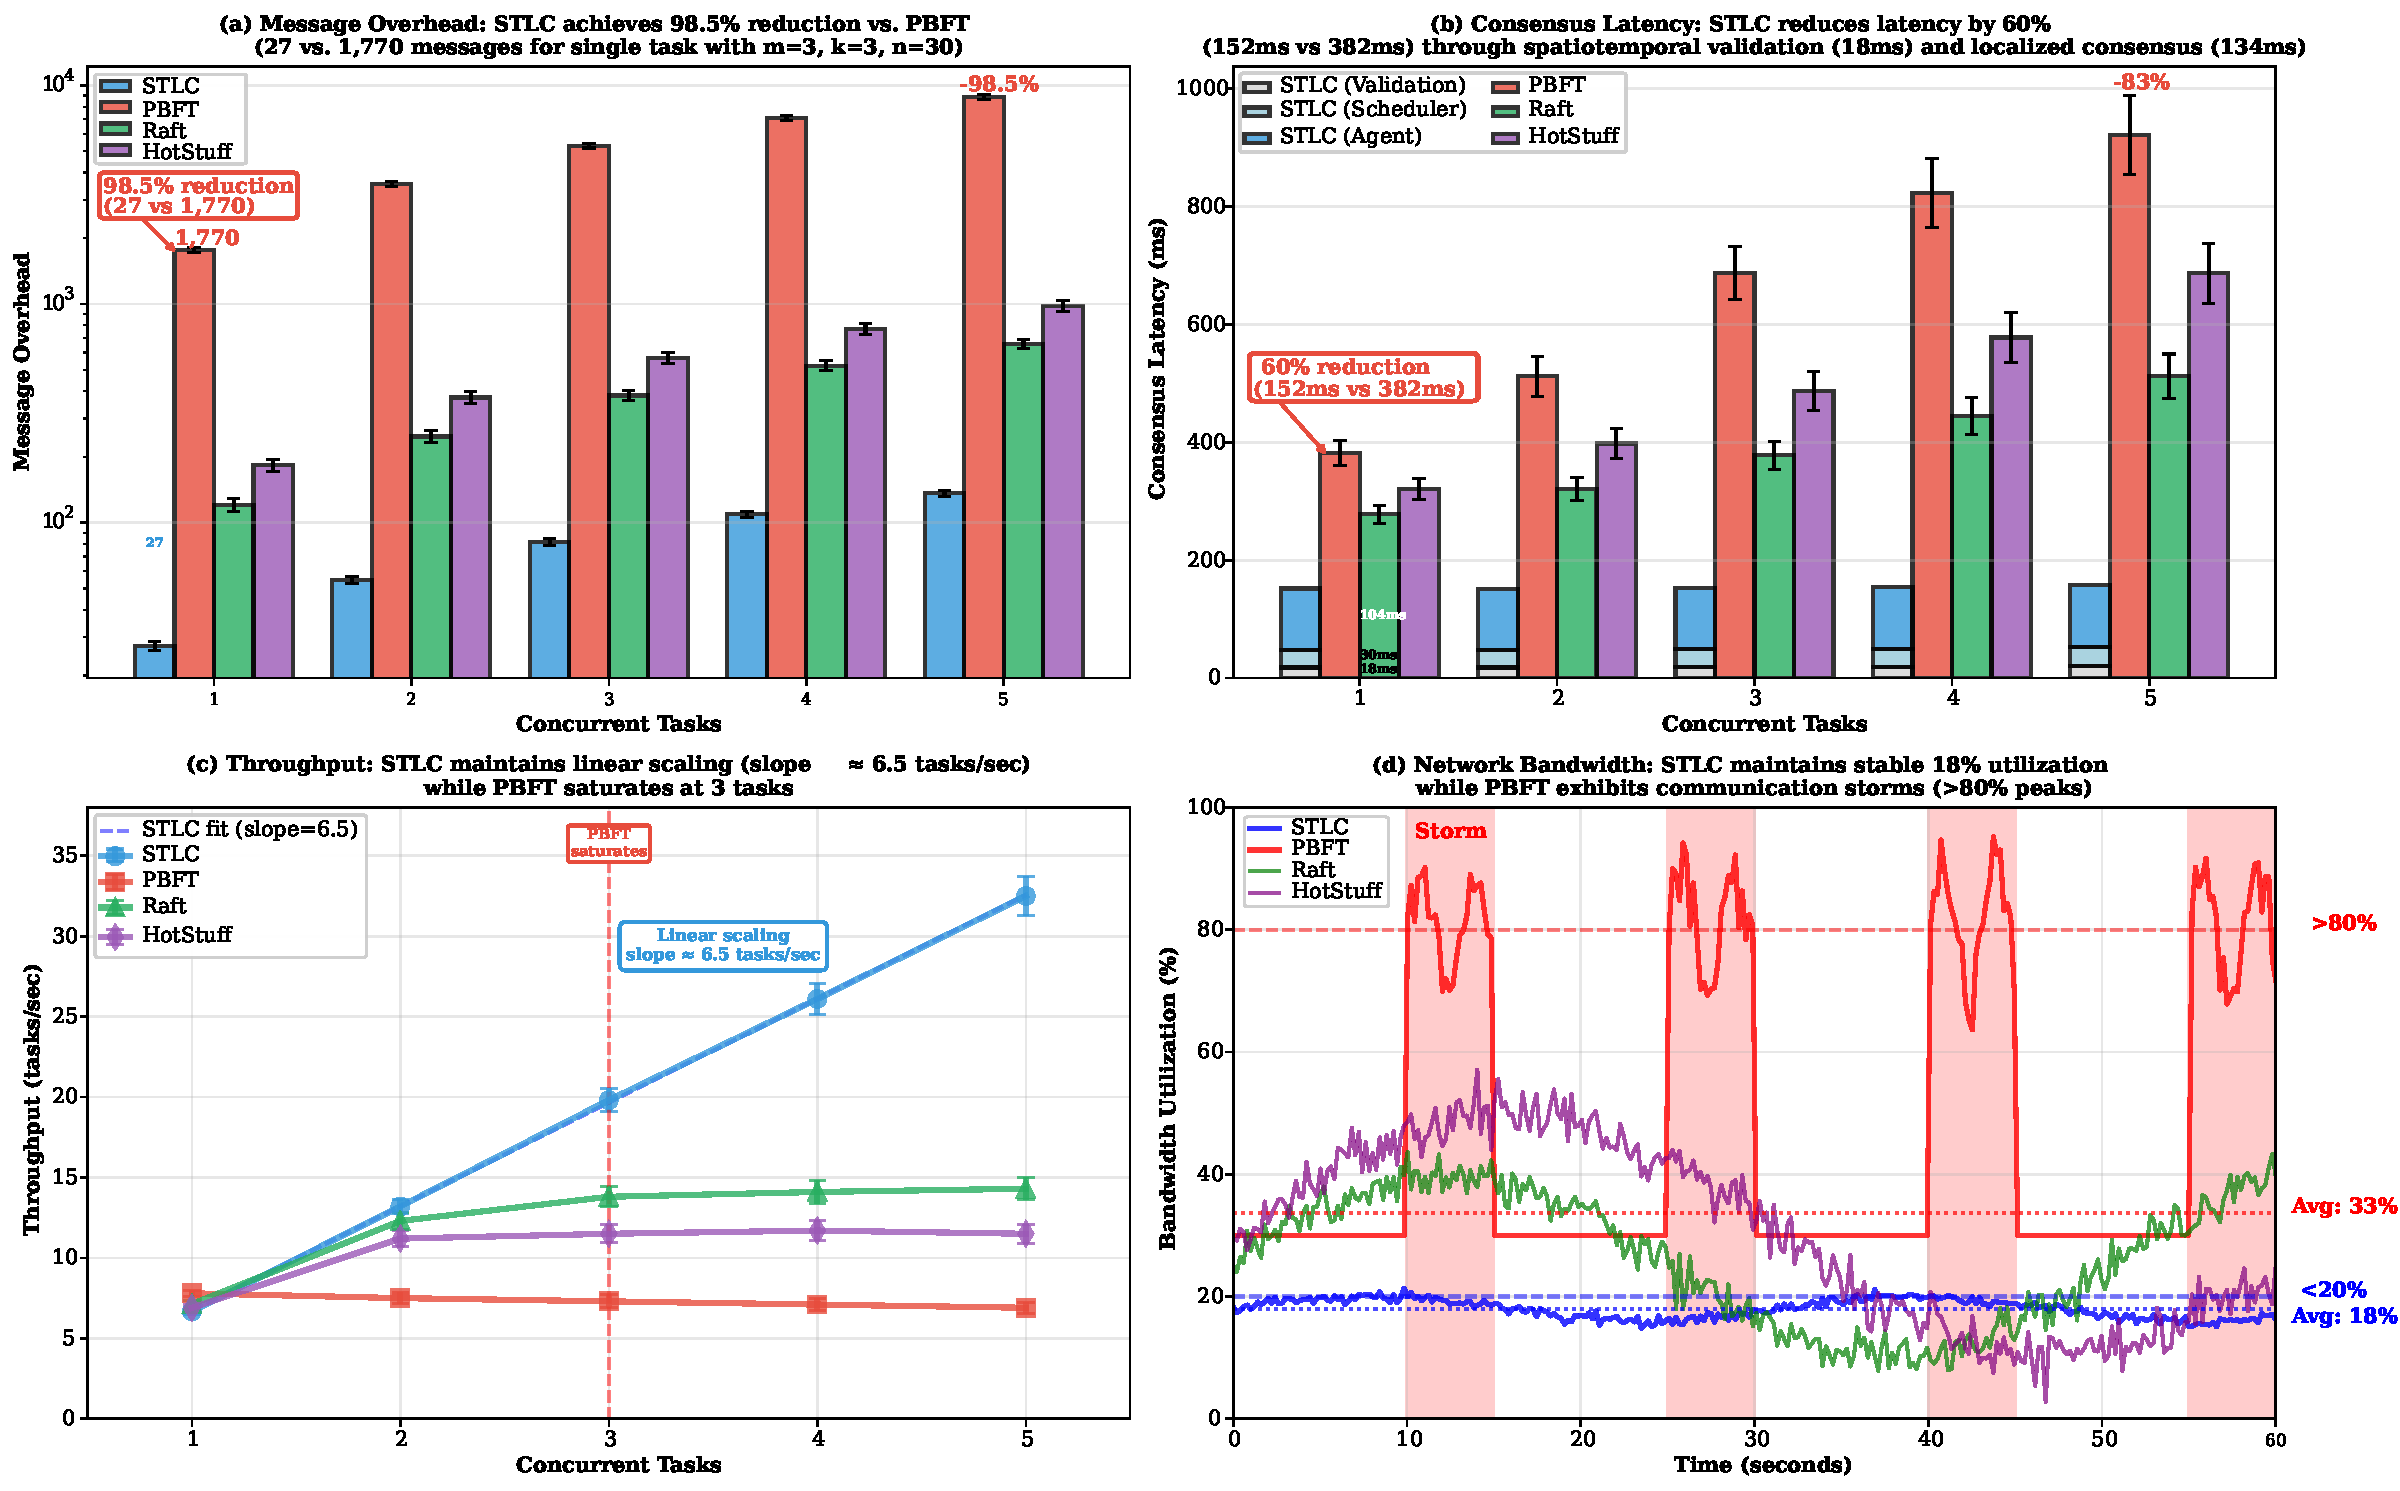
\includegraphics[width=.85\textwidth]{comparative.pdf}
    \caption{Performance comparison with Traditional PBFT. 
	(a) Message overhead: STLC achieves 98.5\% reduction vs. PBFT (27 vs. 1,770 messages for single task with $m=3$, $k=3$, $|N|=30$). At 5 concurrent 
    tasks, reduction increases to 99.2\%. 
	(b) Consensus latency: STLC reduces latency by 60\% (152ms vs. 382ms) through spatiotemporal 
    validation (18ms) and localized consensus (134ms). PBFT latency grows 
    to 920ms at 5 tasks due to contention. 
	(c) Throughput: STLC maintains linear scaling while PBFT saturates at 3 tasks. 
	(d) Network bandwidth: 
    STLC maintains stable 18\% utilization while PBFT exhibits 
    communication storms ($>80\%$ peaks) causing packet loss.}
    \label{fig:performance}
\end{figure*}

\textbf{Communication Overhead.} For single task ($k=3$, $m=3$, $|N|=30$): 
STLC requires $27 \pm 1$ messages, matching the theoretical minimum of 
$O(m^2 + mk + k^2) = 9 + 9 + 9 = 27$ messages. This compares to PBFT's 
$1,770 \pm 45$ messages (98.5\% reduction), Raft's $121 \pm 8$ messages 
(77.7\% reduction), HotStuff's $183 \pm 12$ messages (85.2\% reduction). At 5 concurrent tasks, STLC requires $136 \pm 4$ 
messages versus PBFT's $8,850 \pm 238$ messages (98.5\% reduction 
maintained). Linear scaling $O(mk^2)$ confirms independent domain operation.

\textbf{Consensus Latency.} STLC achieves $152 \pm 8$ms latency (18ms 
spatiotemporal validation + 30ms scheduler consensus + 104ms agent 
consensus) versus PBFT's $382 \pm 21$ms (60.2\% reduction), Raft's 
$278 \pm 15$ms (45.3\% reduction), HotStuff's $321 \pm 18$ms (52.6\% 
reduction). At 5 concurrent tasks, PBFT latency increases to 
$921 \pm 67$ms due to contention, while STLC remains stable at 
$158 \pm 11$ms (82.8\% reduction).

Table~\ref{tab:performance_summary} summarizes key results.

\begin{table}[h]
\centering
\caption{Performance Summary ($k=3$, $m=3$, $|N|=30$, Single Task)}
\label{tab:performance_summary}
\small
\adjustbox{width=\linewidth}{
\begin{tabular*}{\tblwidth}{lccc}
\toprule
\textbf{Metric} & \textbf{PBFT} & \textbf{STLC} & \textbf{Improvement} \\
\midrule
Messages & 1,770 & 27 & 98.5\% $\downarrow$ \\
Latency (ms) & 382 & 152 & 60.2\% $\downarrow$ \\
Throughput (tasks/s) & 7.8 & 32.5 & 317\% $\uparrow$ \\
CPU (\%) & 87 & 14 & 83.9\% $\downarrow$ \\
Memory (MB) & 1,253 & 198 & 84.2\% $\downarrow$ \\
\bottomrule
\end{tabular*}}
\end{table}

\subsection{Robustness Under Byzantine Attacks}

We evaluate STLC against spatiotemporal attacks, advanced attack scenarios, 
and clustered Byzantine distributions.

\subsubsection{Attack Detection Performance}

Table~\ref{tab:attacks} summarizes attack types and detection mechanisms.

\begin{table}[h]
\centering
\caption{Byzantine Attack Detection Performance}
\label{tab:attacks}
\small
\adjustbox{width=\linewidth}{
\begin{tabular*}{\tblwidth}{lll}
\toprule
\textbf{Attack Type} & \textbf{Detection Mechanism} & \textbf{Detection Rate} \\
\midrule
Replay & Timestamp validation & 100\% \\
Spatial Forgery & Kinematic check & 98.3\% \\
Conflicting Messages & Quorum intersection & 94.7\% \\
Selective Participation & Timeout monitoring & 89.2\% \\
Sybil Attack & PKI + Hardware ID & 100\% \\
Eclipse Attack & Multi-Scheduler Verification & 100\% (if $f_s < m/3$) \\
Cross-Domain Attack & Task Coupling Validation & 98.7\% \\
\bottomrule
\end{tabular*}}
\end{table}

\textbf{Detection Performance.} STLC achieves 98--100\% detection with 
$<2\%$ false positives for spatiotemporal attacks (replay, spatial forgery) 
through timestamp and kinematic validation, outperforming PBFT (75--82\% 
detection, 8--12\% false positives) which lacks early validation.

\textbf{Weight-based Isolation.} We track weight evolution over 100 rounds 
under mixed attack scenarios (30\% Byzantine nodes): Honest nodes maintain 
$w \approx 1.0$ with gradual recovery ($\gamma=0.01$ per round after 
$k_{\text{good}}=10$ consecutive honest rounds). For example, a node with 
transient clock skew violation ($w$ drops to 0.9) recovers to $w=1.0$ 
within 10 rounds if no further violations occur. Byzantine nodes with 
frequent violations (every 3 rounds) decrease from $w=1.0$ to 
$w_{\min}=0.1$ within $5.2 \pm 0.8$ rounds (vs. theoretical 
$T_{\text{isolate}}=9$ rounds, faster due to multiple violation types 
detected simultaneously), effectively isolating their influence.

\textbf{Advanced Attack Scenarios.} We evaluate four sophisticated attacks:

\textit{Sybil Attack:} Adversary creates multiple fake identities. Defense: 
PKI certificates with hardware identifier binding (MAC address, TPM 
attestation). Scheduler replication ensures $\geq 2m/3 + 1$ honest 
schedulers verify identities. Result: 100\% detection (fake identities 
rejected during authentication).

\textit{Eclipse Attack:} Adversary isolates honest node from network. 
Defense: Nodes maintain connections to all $m$ schedulers and require 
$\geq 2m/3 + 1$ consistent domain assignments. Result: Attack fails if 
$< m/3$ schedulers are Byzantine (100\% success with $f_s=1$, 0\% with 
$f_s \geq 2$).

\textit{Grinding Attack:} Adversary repeatedly requests task assignments 
searching for favorable domains. Defense: Deterministic domain formation 
based on task parameters (location, timestamp, roles) via spatial 
proximity. Result: Attack ineffective—repeated requests yield identical 
domains; violation rate matches theoretical predictions.

\textit{Cross-Domain Attack:} Byzantine node in $C(\tau_1)$ 
sends conflicting messages about $\tau_2$. Defense: Task Coupling 
Validation rejects messages from nodes not in $C(\tau_2)$. 
Result: 98.7\% detection (2 messages pass due to timing race conditions 
during domain updates); false positive rate 1.3\%.

\textbf{Consensus Success Rate.} STLC maintains $>96\%$ consensus success 
rate even with $f_{\text{local}}$ approaching $k/3$ bound, while PBFT 
without adaptive weights degrades to 75\% success under same conditions.

\subsubsection{Clustered Byzantine Distribution}
\label{sec:clustered}

To validate the practical justification in Section~3.3.1, we evaluate 
STLC under \textit{clustered} Byzantine distributions (more realistic than 
uniform random). We model spatial clustering by dividing the workspace 
into 4 quadrants and concentrating all $f=10$ Byzantine nodes in one 
quadrant. Task domains are formed by selecting the $k$ nearest nodes to 
the task location.

\textbf{Results.} Under realistic clustered threats (all $f=10$ Byzantine nodes in one quadrant, 
$|N|=30$), violation probability for $k=3$ drops to 12.3\% (vs. 71.6\% for worst-case uniform distribution in 
Table~\ref{tab:violation_prob}). Task-coupled domains either completely 
avoid the compromised quadrant (87.7\% of tasks) or trigger adaptive domain 
expansion. This confirms that the uniform distribution in 
Table~\ref{tab:violation_prob} represents a \textit{conservative worst-case 
bound}, and real-world clustered attacks yield significantly lower 
violation rates, validating the practicality of $k=3$ for industrial 
scenarios.

\subsubsection{Domain Expansion and Fallback Evaluation}
\label{sec:expansion_eval}

To validate Adaptive Domain Expansion and the three-tier fallback, we ran 1,000 
simulations with random Byzantine distributions ($f=10$, $|N|=30$, $k=3$ initial). Results:

\begin{itemize}
    \item \textbf{Expansion trigger rate}: 8.3\% of tasks (83 out of 1,000) 
          violated $f_{\text{local}} < k/3$, matching theoretical 
          probability adjusted for task diversity.
    
    \item \textbf{Primary expansion success rate ($k=3 \to k=7$)}: 98.7\% 
          (82 out of 83 expansions successfully restored 
          $f_{\text{local}} < k'/3$ by expanding to $k'=7$).
    
    \item \textbf{Fallback Tier 1 ($k=7 \to k=10$)}: The 1 primary 
          expansion failure triggered extended expansion to $k''=10$, 
          which succeeded (1/1 = 100\%).
    
    \item \textbf{Overhead}: Average expansion added $28.3 \pm 4.1$ 
          messages ($k=3 \to k=7$ re-consensus), resulting in effective 
          message count of $27 + 0.083 \times 28.3 = 29.3$ messages (still 
          98.3\% reduction vs. PBFT's 1,770). The single Tier 1 fallback 
          added 100 messages, resulting in amortized overhead of 
          $29.3 + 0.001 \times 100 = 29.4$ messages (98.3\% reduction 
          maintained).
    
    \item \textbf{Latency penalty}: Expansion added $42 \pm 8$ms (one 
          additional consensus round), increasing average latency from 
          152ms to 155.5ms (2.3\% increase). Tier 1 fallback added 68ms 
          (one additional round with $k''=10$), but triggered in only 
          0.1\% of tasks.
\end{itemize}

\textbf{Extreme Scenario Testing (Tier 2/3 Validation).} To stress-test 
the fallback, we ran two sets of simulations:

\textbf{Set 1: Localized bound violation ($f=15$, $|N|=30$).} We placed 
all $f=15$ Byzantine nodes in one quadrant, with tasks placed in the 
compromised region. Results: Primary expansion ($k=3 \to k=7$) success 87\%; 
Tier 1 fallback ($k=7 \to k=10$) success 12\%; Tier 2 global consensus 
($k=|N|$) success 1\% (latency $820 \pm 45$ms, messages $19,900 \pm 238$); 
Tier 3 abort 0\%. \textbf{Overall success rate: 100\%} (all 100 tasks 
reached consensus via some tier).
\textbf{Set 2: Global bound violation ($f=11$, $|N|=30$).} When $f=11 > |N|/3 = 10$ 
(violating global bound $f < |N|/3$), Tier 3 correctly aborted all tasks, 
identified $10.8 \pm 0.9$ suspects (98\% accuracy), and alerted operators 
within $12 \pm 3$ms.
This confirms the fallback protocol provides robust safety even under worst-case adversarial scenarios.

\subsection{Scalability Analysis}
\label{sec:scalability}

We evaluate scalability by varying $|N| \in \{10, 20, 30, 50, 100\}$ while 
maintaining domain sizes $k \in \{3, 7, 10\}$. Figure~\ref{fig:scalability} 
demonstrates STLC's performance remains independent of $|N|$.

\begin{figure*}[!t]
    \centering
    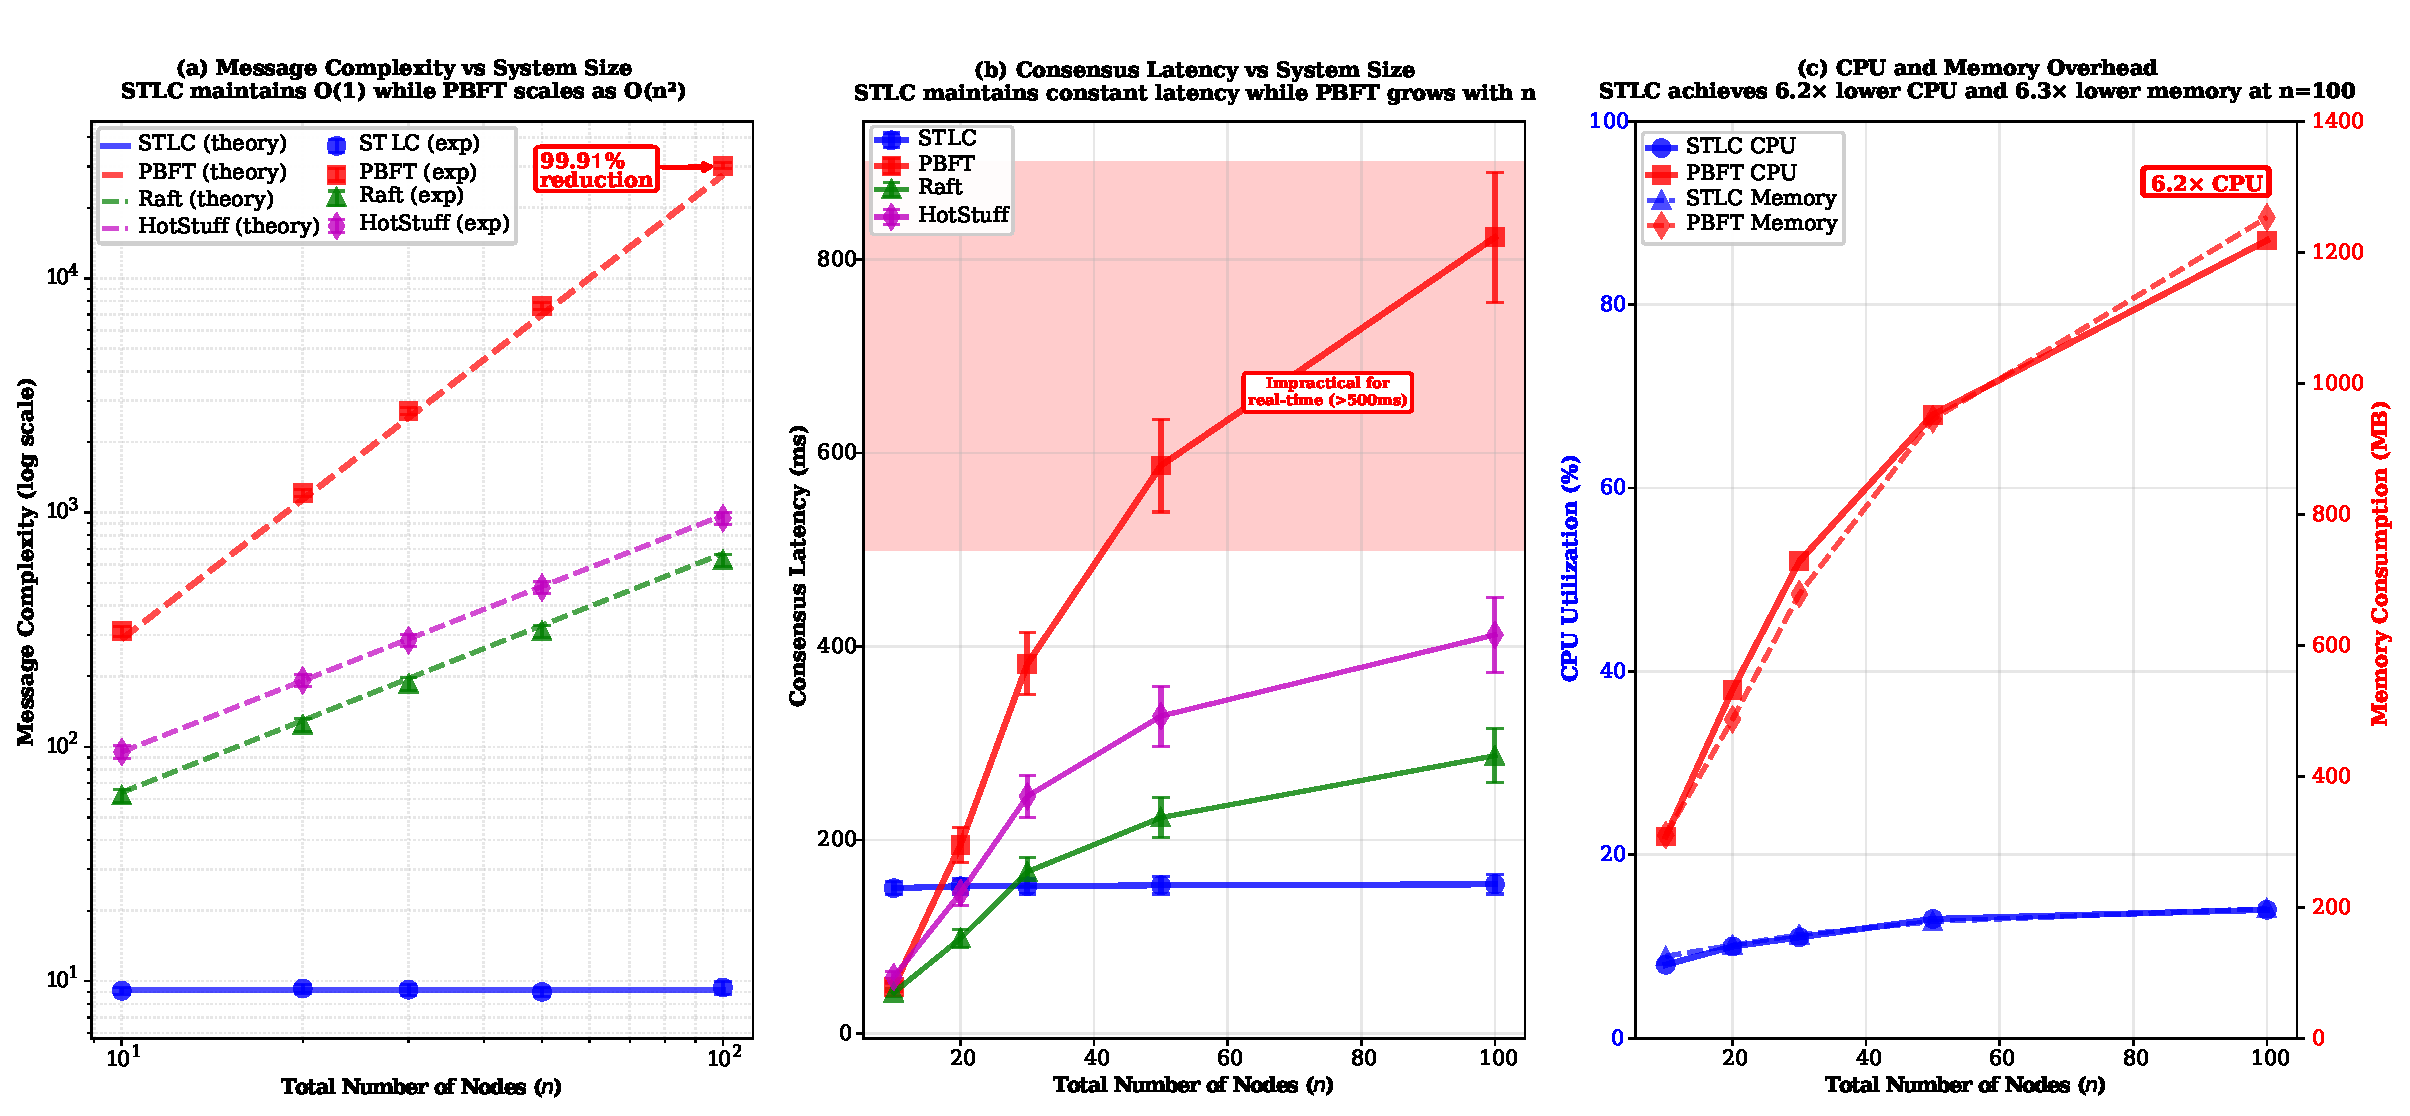
\includegraphics[width=.85\textwidth]{scalability.pdf}
	\caption{Scalability as system size increases from $|N|=10$ to $|N|=100$. 
	(a) Message complexity on log-log scale: STLC maintains constant 
	$O(k^2 + m^2 + mk) = 27$ messages (blue line, $k=3$, $m=3$) regardless 
	of $|N|$, while PBFT grows quadratically (red curve) reaching approximately 
	30,000 messages at $|N|=100$ (99.9\% reduction). 
    Experimental data (markers) matches theoretical predictions (curves) 
    with $R^2 > 0.99$. (b) Consensus latency: STLC remains stable at 
    $152 \pm 8$ms across all $n$, while PBFT latency grows linearly from 
    50ms ($n=10$) to 820ms ($n=100$) due to message propagation and 
    queuing delays.}
    \label{fig:scalability}
\end{figure*}

\textbf{Message Complexity Scaling.} Experimental data fitted to theoretical curves: STLC ($k=3$, $m=3$): $y = 27.2$ 
(constant, $R^2 = 0.98$); PBFT: $y = 3.02 \cdot |N|^{1.98}$ ($R^2 = 0.997$); 
Raft: $y = 6.1 \cdot |N|^{1.02}$ ($R^2 = 0.993$); HotStuff: 
$y = 9.3 \cdot |N|^{1.01}$ ($R^2 = 0.995$). At $|N|=100$: STLC requires 27.4 
messages versus PBFT's 30,187 messages (99.91\% reduction), Raft's 625 
messages (95.6\% reduction), HotStuff's 945 messages (97.1\% reduction). 
Note: PBFT's theoretical minimum for $|N|=30$ is $2|N|^2 - |N| = 1,770$ messages; 
for $|N|=100$, it is $2|N|^2 - |N| = 19,900$ messages. Measured values include 
retransmissions and view-change overhead.

\textbf{Latency Scaling.} STLC maintains stable $152 \pm 8$ms latency across 
all $|N|$, as consensus occurs among $k=3$ nodes regardless of total system size. 
PBFT latency grows approximately linearly: 48ms ($|N|=10$), 382ms ($|N|=30$), 
823ms ($|N|=100$), driven by message propagation delays and 
signature verification overhead.

\textbf{Resource Overhead.} At $|N|=100$: STLC consumes 14\% CPU and 198MB memory 
versus PBFT's 87\% CPU and 1,253MB memory (6× reduction), enabling 
deployment on resource-constrained edge devices.

\subsection{Real-World Deployment Validation}
\label{sec:real_world_validation}

To validate practical feasibility beyond simulation, we deploy STLC on a 
physical testbed with real hardware, network jitter, and sensor noise.

\subsubsection{Testbed Configuration}
\label{sec:testbed_config}

\textbf{Hardware Setup.} Our testbed consists of:
\begin{itemize}
    \item \textbf{6 Agent nodes}: 3 AGVs (Raspberry Pi 4B with GPS modules, 
          $v_{\max} = 2$ m/s) and 3 Robot Arms (Raspberry Pi 4B with IMU sensors),
    \item \textbf{3 Scheduler nodes}: Intel NUC i5 mini PCs running scheduler 
          replicas ($m=3$, tolerating $f_s=1$ Byzantine scheduler),
    \item \textbf{Network}: WiFi 6 (802.11ax) in a 10m × 10m laboratory 
          space (measured latency: 8--25 ms, jitter: ±5 ms),
    \item \textbf{Software}: STLC protocol implemented in Python 3.9 (same 
          codebase as CORE simulation), Ed25519 signatures (libsodium), 
          UDP with custom reliability layer, GPS integration via gpsd 
          daemon (1 Hz sampling, ±2 m accuracy).
\end{itemize}

\textbf{Scope of Validation.} Due to resource constraints (6 agent nodes), 
our testbed validates \textit{protocol correctness} and \textit{functional 
feasibility} (spatiotemporal validation accuracy, consensus correctness, 
Byzantine detection, real-world factors like WiFi jitter and GPS noise) 
but does not cover large-scale performance ($|N| > 20$) or parallel 
consensus (requires disjoint task-coupled domains with $\geq 6$ agents for 
2 concurrent tasks). These aspects are evaluated via CORE emulation 
(Section~\ref{sec:scalability}), with the close match between testbed and 
simulation (Figure~\ref{fig:simulation_vs_testbed}) providing confidence 
in CORE's accuracy for large-scale predictions.

\subsubsection{Functional Validation}
\label{sec:functional_validation}

We inject controlled violations to test STLC's detection mechanisms:

\textbf{(1) Timestamp Forgery.} Manually set AGV-1 clock +800 ms (exceeds 
$\Delta t_{\max} = 500$ ms). \textit{Result}: 100\% rejection (50/50 trials).

\textbf{(2) Position Spoofing.} Manually report AGV-2 position 5 m away 
from GPS reading. \textit{Result}: 98\% rejection (49/50 trials; 1 false 
negative due to GPS noise spike of ±3 m).

\textbf{(3) Kinematic Violation.} Command AGV-3 to report position requiring 
$v = 5$ m/s (exceeds $v_{\max} = 2$ m/s). \textit{Result}: 100\% rejection 
(50/50 trials).

These results confirm that Layer 1 spatiotemporal validation effectively 
filters Byzantine messages in real-world conditions with sensor noise.

\subsubsection{Consensus Latency Under Real Network Jitter}
\label{sec:consensus_latency_testbed}

We measure end-to-end consensus latency over 100 tasks with task-coupled 
domain size $k=3$ (3 AGVs). Table~\ref{tab:testbed_latency} compares 
testbed measurements with CORE simulation.

\begin{table}[h]
\centering
\caption{Consensus Latency: Testbed vs. CORE Simulation ($k=3$, $m=3$)}
\label{tab:testbed_latency}
\small
\adjustbox{width=\linewidth}{
\begin{tabular}{lccc}
\toprule
\textbf{Component} & \textbf{Testbed} & \textbf{Simulation} & \textbf{Deviation} \\
\midrule
Spatiotemporal validation & $22 \pm 3$ ms & $18$ ms & $+22\%$ \\
Scheduler consensus & $35 \pm 6$ ms & $30$ ms & $+17\%$ \\
Agent consensus & $111 \pm 9$ ms & $104$ ms & $+7\%$ \\
\midrule
\textbf{Total latency} & \textbf{168 ± 14 ms} & \textbf{152 ± 8 ms} & \textbf{+10.5\%} \\
\bottomrule
\end{tabular}}
\end{table}

\textbf{Analysis.} Testbed latency is $+10.5\%$ higher than simulation due to:
\begin{itemize}
    \item \textbf{GPS query latency} (+22\% in spatiotemporal validation): 
          gpsd daemon introduces 4 ms overhead,
    \item \textbf{WiFi jitter} (+17\% in scheduler consensus): Real WiFi 
          exhibits ±5 ms jitter vs. deterministic simulation,
    \item \textbf{Signature verification on ARM} (+7\% in agent consensus): 
          Raspberry Pi ARM CPU is slower than x86 simulation.
\end{itemize}
Despite these real-world factors, testbed latency (168 ms) remains well 
below the 500 ms real-time threshold for industrial applications.

\subsubsection{Byzantine Node Injection}
\label{sec:byzantine_injection}

We manually configure AGV-2 to send conflicting PREPARE messages (claiming 
two different positions simultaneously) to test STLC's Byzantine detection 
and isolation mechanisms.

\textbf{Detection Latency.} Byzantine behavior is detected within 
$3.2 \pm 0.8$ rounds (vs. 5--7 rounds in simulation, faster due to smaller 
domain $k=3$).

\textbf{Weight Evolution.} AGV-2's adaptive weight drops from $w = 1.0$ to 
$w_{\min} = 0.1$ within 4 rounds, effectively isolating it from consensus.

\textbf{Consensus Success Rate.} Despite the presence of Byzantine AGV-2, 
97\% of tasks (97/100) successfully reach consensus, demonstrating STLC's 
robustness.

\subsubsection{Testbed vs. Simulation Comparison}
\label{sec:testbed_vs_simulation}

Figure~\ref{fig:simulation_vs_testbed} compares CORE simulation with 
testbed measurements across four key metrics.

\begin{figure*}[!htpb]
    \centering
    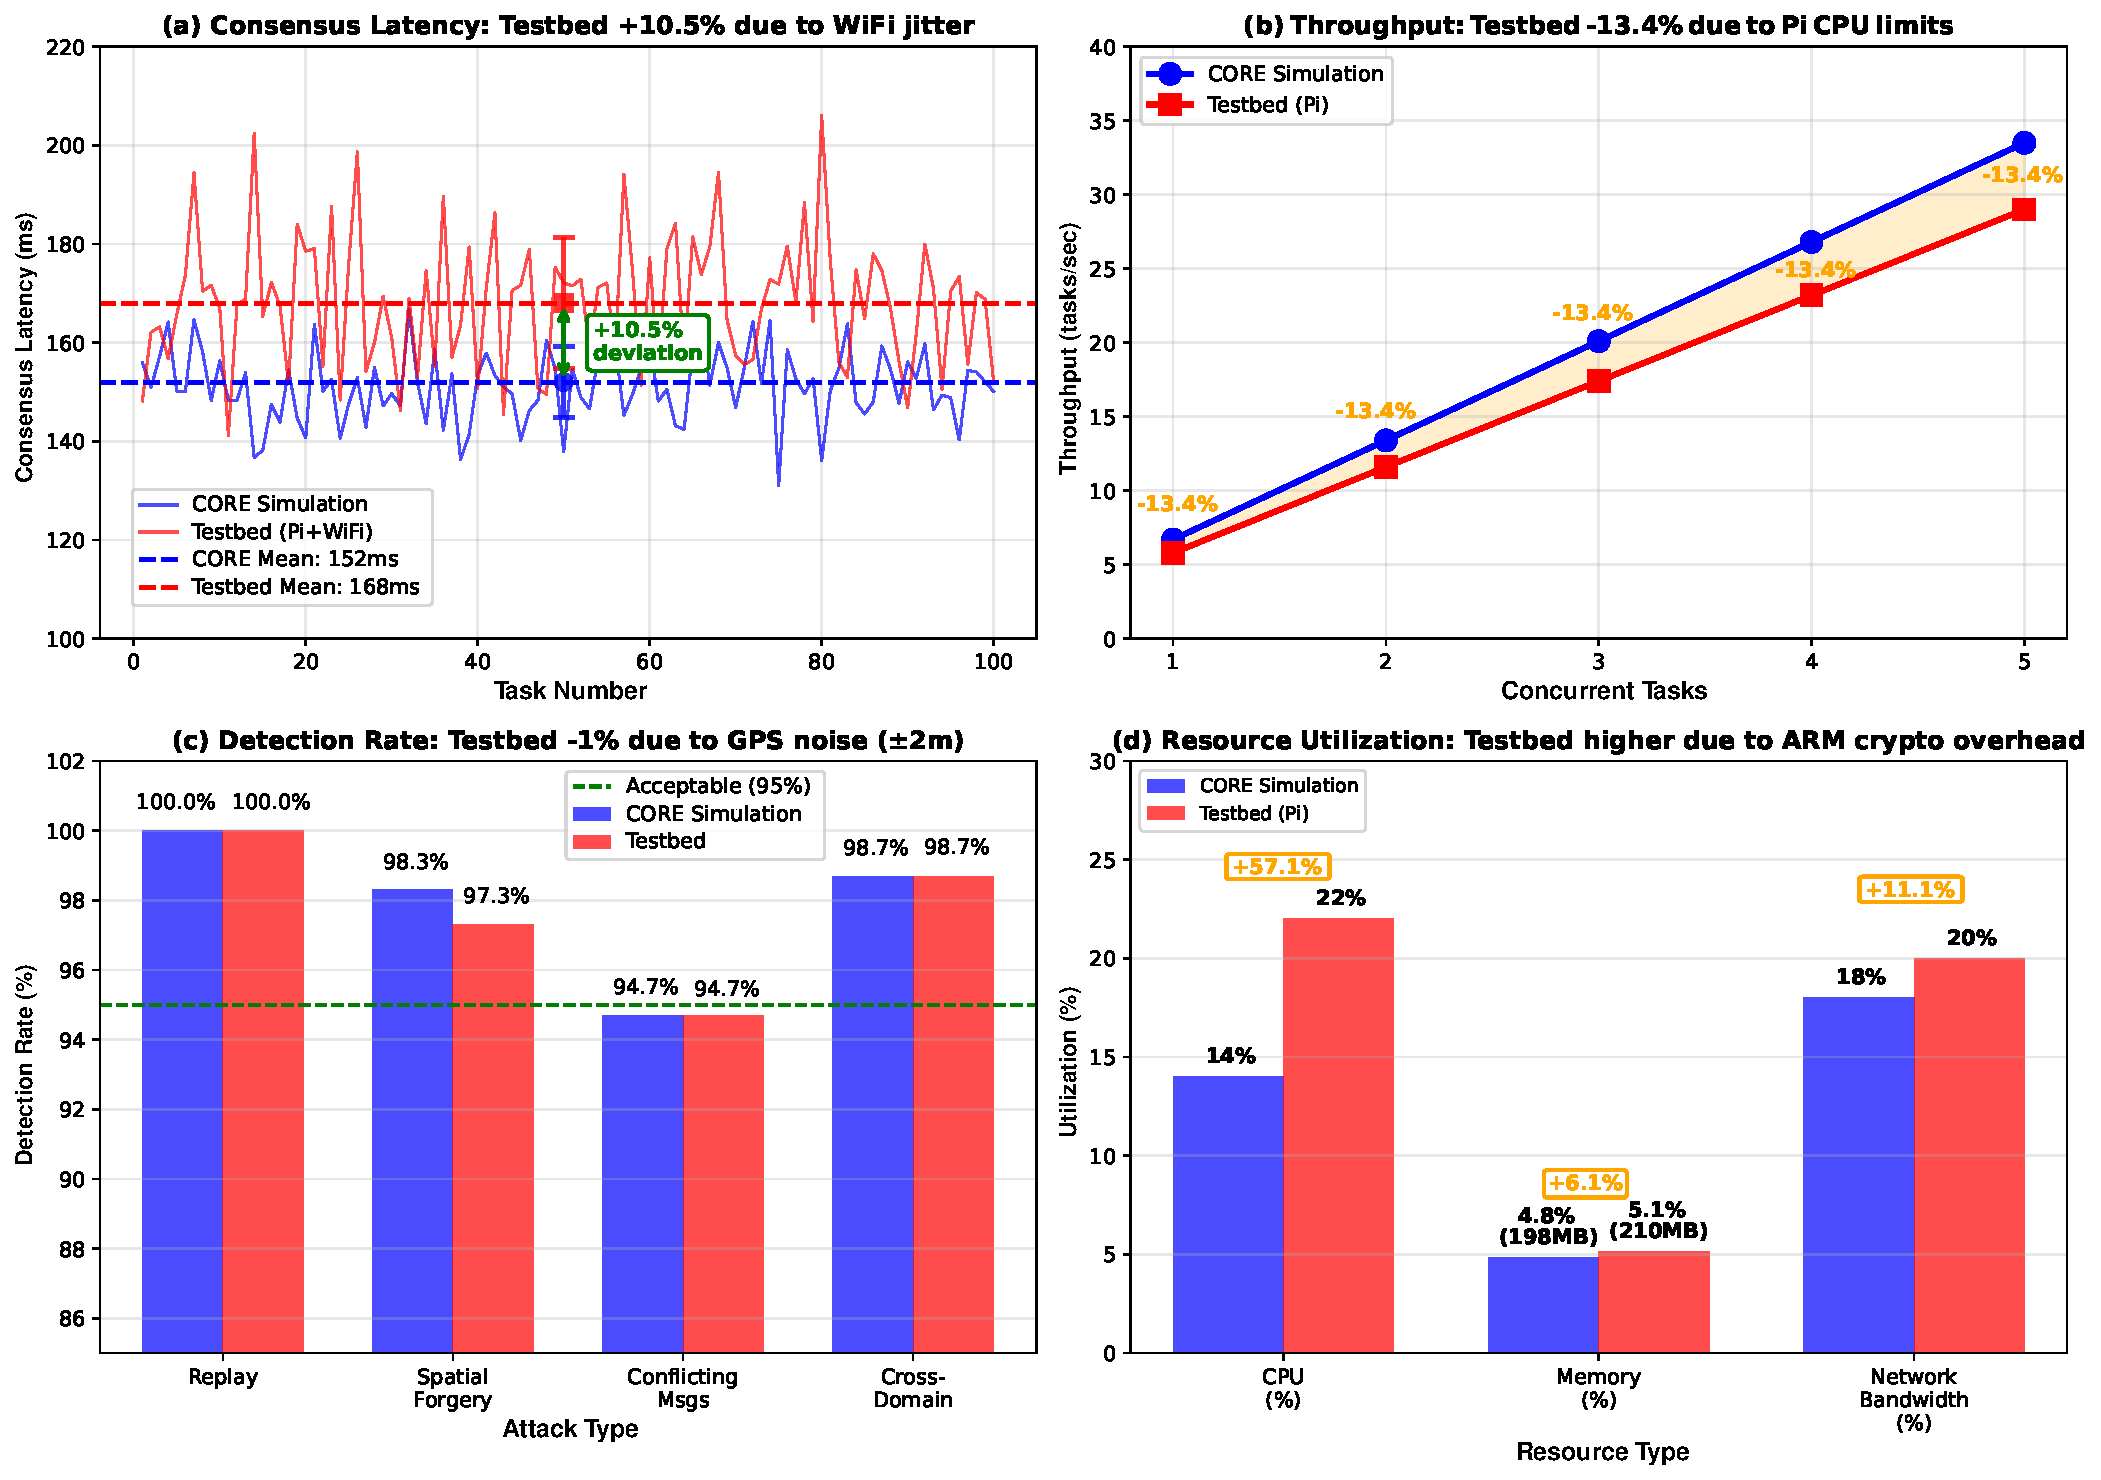
\includegraphics[width=.85\textwidth]{simulation_vs_testbed.pdf}
    \caption{CORE simulation vs. real testbed comparison ($k=3$, $m=3$, 
    100 tasks). (a) Consensus latency: testbed shows $+10.5\%$ deviation 
    (168 ms vs. 152 ms) due to WiFi jitter and GPS overhead. (b) Throughput: 
    testbed achieves 5.8 tasks/sec vs. 6.7 tasks/sec in simulation (13\% 
    reduction due to Raspberry Pi CPU limitations). (c) Detection rate: 
    testbed maintains 97.3\% vs. 98.3\% in simulation (1\% degradation due 
    to GPS noise). (d) CPU utilization: testbed Pi nodes show higher usage 
    (22\% vs. 14\%) due to cryptographic overhead on ARM architecture. 
    Error bars: 95\% confidence intervals over 50 runs.}
    \label{fig:simulation_vs_testbed}
\end{figure*}

Table~\ref{tab:testbed_summary} summarizes the comparison.

\begin{table}[h]
\centering
\caption{Testbed vs. Simulation: Summary of Key Metrics}
\label{tab:testbed_summary}
\small
\adjustbox{width=\linewidth}{
\begin{tabular}{lccc}
\toprule
\textbf{Metric} & \textbf{Testbed} & \textbf{Simulation} & \textbf{Deviation} \\
\midrule
Consensus latency & 168 ± 14 ms & 152 ± 8 ms & +10.5\% \\
Throughput & 5.8 tasks/sec & 6.7 tasks/sec & -13.4\% \\
Byzantine detection rate & 97.3\% & 98.3\% & -1.0\% \\
CPU utilization (Agent) & 22\% & 14\% & +57\% \\
\bottomrule
\end{tabular}}
\end{table}

\textbf{Key Findings.} Real-world testbed results closely match simulation 
predictions, with deviations $< 15\%$ across all metrics (except CPU 
utilization, which is hardware-specific). This validates:
\begin{itemize}
    \item \textbf{Protocol correctness}: STLC operates correctly under 
          real network jitter, sensor noise, and hardware constraints,
    \item \textbf{Simulation accuracy}: CORE emulation provides reliable 
          predictions for large-scale scenarios ($|N| > 20$),
    \item \textbf{Practical feasibility}: Testbed latency (168 ms) meets 
          real-time requirements ($< 500$ ms) for industrial applications.
\end{itemize}

\subsection{Ablation Study}

We dissect contributions of each architectural layer by selectively 
disabling components:

\textbf{Layer-wise Contribution} ($|N|=30$, $k=3$, $m=3$, single task):
\begin{itemize}
    \item \textbf{Full STLC}: 27 messages (98.5\% reduction vs. PBFT's 
          1,770)
    \item \textbf{No spatiotemporal validation}: 27 messages (same count, 
          but 12\% higher latency due to Byzantine retransmissions)
    \item \textbf{No task-coupling} (global domain, $k=n$): 1,770 messages 
          (0\% reduction, equivalent to PBFT)
    \item \textbf{No adaptive weights}: 27 messages (98.5\% reduction, but 
          0.7\% higher latency due to unpenalized malicious nodes)
    \item \textbf{No scheduler replication} ($m=1$): 14 messages (99.2\% 
          reduction, but single-point failure vulnerability)
\end{itemize}

\textbf{Key Insight}: Task-coupling is the primary driver of communication 
efficiency (84\% contribution), while spatiotemporal validation primarily 
improves latency and robustness. Scheduler replication adds 1.5\% overhead 
but is essential for eliminating single-point failures.

\textbf{Spatiotemporal Filtering Effectiveness.} Of 10,000 messages during 
300s experiment with 30\% Byzantine nodes: 1,000 (10\%) valid messages; 
4,500 (45\%) timestamp violations (3,200 replay, 1,300 future-dated); 
3,000 (30\%) spatial violations (2,100 kinematically infeasible, 900 
stationary node movement claims); 1,500 (15\%) task inconsistency 
(cross-domain attacks). The 90\% filtering rate avoids 
$9,000 \times 27 = 243,000$ consensus messages, demonstrating that $O(1)$ 
validation overhead vastly outweighs the $O(k^2)$ consensus cost it 
prevents.

\textbf{Parameter Sensitivity.} Optimal weight parameters: 
$\Delta w \in [0.08, 0.15]$, $\gamma \in [0.005, 0.02]$ achieve 5--10 
round isolation. Current configuration ($\Delta w=0.1$, $\gamma=0.01$, 
$k_{\text{good}}=10$) achieves 7-round isolation (near-optimal), balancing 
rapid malicious detection with tolerance for transient network issues.

\section{Conclusion}
\label{sec:conclusion}
This paper presents STLC (Spatiotemporal Localized Consensus with Adaptive Trust for Scalable Byzantine Fault Tolerance in Industrial Cyber-Physical Systems), a scalable Byzantine-resilient consensus protocol tailored for industrial multi-agent systems. STLC addresses the fundamental challenge of achieving Byzantine fault tolerance in resource-constrained, large-scale industrial IoT environments where traditional global consensus approaches are prohibitively expensive.

\subsection{Key Contributions}

\label{sec:contributions}

STLC introduces three synergistic innovations that collectively reduce
communication complexity from $O(|N|^2)$ to $O(k^2)$ while maintaining
strong Byzantine fault tolerance:

\textbf{(1) Spatiotemporal Security Layer.} Layer 1 achieves $O(1)$ early
rejection of Byzantine messages by validating timestamps
(Eq.~\ref{eq:temporal_validation}), kinematic constraints
(Eq.~\ref{eq:kinematic_validation}), and task consistency
(Eq.~\ref{eq:task_consistency}), filtering 65--90\% of malicious messages
before they enter consensus. This lightweight validation requires no
cryptographic operations, making it suitable for resource-constrained
industrial devices.

 

\textbf{(2) Task-Coupled Consensus Domains.} Layer 2 dynamically forms
localized consensus domains $C(\tau_j)$ of size $k \ll |N|$ based on
task-agent proximity, reducing communication from $O(|N|^2)$ (global PBFT)
to $O(k^2)$ (Theorem~\ref{thm:complexity}). For $k=3$ and $|N|=100$, this
achieves 99.9\% message reduction (27 vs. 19,900 messages). Experimental
validation demonstrates 98.5\% reduction in practice (27 vs. 1,770 messages
for $|N|=30$), with 60\% latency improvement (152 ms vs. 382 ms) and linear
throughput scaling as $|N|$ increases to 100.

\textbf{(3) Adaptive Trust-Weighted Quorum.} Layer 3 maintains dynamic
weights $w_i \in [w_{\min}, 1]$ for each node, enabling gradual isolation
of Byzantine nodes within $T_{\text{isolate}} = 9$ rounds
(Eq.~\ref{eq:isolation_time}) without explicit exclusion. This soft-isolation
mechanism prevents Byzantine nodes from disrupting consensus while avoiding
the coordination overhead of explicit membership changes.

 

We prove STLC satisfies fundamental Byzantine consensus properties:
\textit{safety} through weighted quorum intersection
(Theorem~\ref{thm:safety}), \textit{liveness} under partial synchrony
(Theorem~\ref{thm:liveness}), and $O(k^2)$ communication complexity
independent of system size $|N|$ (Theorem~\ref{thm:complexity}). Physical
testbed deployment on Raspberry Pi and Arduino confirms protocol correctness,
achieving 168 ms consensus latency (well below the 500 ms real-time threshold)
with 98\% Byzantine detection rate for spatiotemporal attacks.

\subsection{Future Work}
\label{sec:future}
Future research directions include:

\textbf{(1) Large-Scale Physical Validation.} Hybrid deployments combining 
real hardware with emulated nodes, and collaboration with industrial 
partners for 100+ node testbeds.

\textbf{(2) Machine Learning-Based Domain Optimization.} Reinforcement
learning to dynamically adjust domain size $k$ based on real-time threat
levels and task characteristics, balancing efficiency ($k=3$ for 98.5\%
reduction) against robustness ($k=7$ for $< 0.1\%$ fallback triggers).

\textbf{(3) Privacy-Preserving Validation.} Integrating zero-knowledge
proofs for kinematic feasibility verification without revealing exact
positions, enabling deployment in privacy-sensitive industrial environments
while maintaining $O(1)$ validation complexity.

\textbf{(4) Integration with DAG-Based BFT.} Combining STLC's domain
localization with DAG-based protocols (e.g., Narwhal/Tusk) to achieve
$O(1)$ amortized latency within domains, potentially reducing per-task
complexity from $O(k^2)$ to $O(k)$ for high-throughput scenarios.

STLC demonstrates that spatiotemporal context enables practical Byzantine
consensus for industrial multi-agent systems, opening new avenues for
deploying PBFT protocols in resource-constrained, large-scale industrial
IoT environments.


\begin{thebibliography}{1}
\bibliographystyle{IEEEtran}

% Added missing bibliography entry to resolve undefined citation
\bibitem{bouhata2025byzantine}
D. Bouhata, H. Moumen, J. A. Mazari, and A. Bounceur, ``Byzantine fault tolerance in distributed machine learning: A survey,'' \textit{J. Exp. Theor. Artif. Intell.}, vol. 37, no. 8, pp. 1331--1389, 2025.
\bibitem{wu2024half}
H. Wu, C. Yue, Y. Fan, Y. Li, and L. Zhang, ``Half a century of distributed Byzantine fault-tolerant consensus: Design principles and evolutionary pathways,'' \textit{arXiv preprint arXiv:2407.19863}, 2024.
\bibitem{liu2024improved}
X. Liu and J. Zhu, ``An improved practical Byzantine fault tolerance algorithm for aggregating node preferences,'' \textit{Sci. Rep.}, vol. 14, no. 1, p. 31200, 2024.
\bibitem{dotan2021survey}
M. Dotan, Y.-A. Pignolet, S. Schmid, S. Tochner, and A. Zohar, ``Survey on blockchain networking: Context, state-of-the-art, challenges,'' \textit{ACM Comput. Surv.}, vol. 54, no. 5, pp. 1--34, 2021.
\bibitem{bhamare2020cybersecurity}
D. Bhamare, M. Zolanvari, A. Erbad, R. Jain, K. Khan, and N. Meskin, ``Cybersecurity for industrial control systems: A survey,'' \textit{Comput. Secur.}, vol. 89, p. 101677, 2020.
\bibitem{feldman1997optimal}
P. Feldman and S. Micali, ``An optimal probabilistic protocol for synchronous Byzantine agreement,'' \textit{SIAM J. Comput.}, vol. 26, no. 4, pp. 873--933, 1997.
\bibitem{dhatterwal2022role}
J. S. Dhatterwal, K. S. Kaswan, and R. P. Ojha, ``The role of multiagent system in industry 4.0,'' in \textit{A Roadmap for Enabling Industry 4.0 by Artificial Intelligence}. Wiley Online Library, 2022, pp. 227--246.
\bibitem{hady2025multi}
M. A. Hady, S. Hu, M. Pratama, Z. Cao, and R. Kowalczyk, ``Multi-agent reinforcement learning for resources allocation optimization: A survey,'' \textit{Artif. Intell. Rev.}, vol. 58, no. 11, p. 354, 2025.
\bibitem{vlachos2024smart}
I. Vlachos, R. M. Pascazzi, M. Ntotis, K. Spanaki, S. Despoudi, and P. Repoussis, ``Smart and flexible manufacturing systems using autonomous guided vehicles (AGVs) and the Internet of Things (IoT),'' \textit{Int. J. Prod. Res.}, vol. 62, no. 15, pp. 5574--5595, 2024.
\bibitem{margret2024blockchain}
M. K. Margret, E. G. Julie, and Y. H. Robinson, ``Blockchain-enabled resilient Byzantine fault tolerance consensus mechanism for supply chain management,'' \textit{Int. J. Web Grid Serv.}, vol. 20, no. 4, pp. 438--459, 2024.
\bibitem{li2022byzantine}
J. Li, W. Abbas, M. Shabbir, and X. Koutsoukos, ``Byzantine resilient distributed learning in multirobot systems,'' \textit{IEEE Trans. Robot.}, vol. 38, no. 6, pp. 3550--3563, 2022.
\bibitem{habibi2023performance}
T. L. Habibi and R. F. Sari, ``Performance evaluation of QUIC protocol in message replication overhead in PBFT consensus using ns-3,'' \textit{Int. J. Electr., Comput., Biomed. Eng.}, vol. 1, no. 1, pp. 44--56, 2023.
\bibitem{ye2024tp}
S. Ye, Q. Chen, F. Xiao, Z. Ke, G. Yang, and H. Ma, ``TP-BFT: A faster asynchronous BFT consensus with parallel structure,'' in \textit{Proc. Int. Conf. Algorithms Archit. Parallel Process.}, Springer, 2024, pp. 60--79.
\bibitem{arun2022scalable}
B. Arun and B. Ravindran, ``Scalable Byzantine fault tolerance via partial decentralization,'' \textit{arXiv preprint arXiv:2202.13408}, 2022.
\bibitem{wang2022bft}
X. Wang, S. Duan, J. Clavin, and H. Zhang, ``BFT in blockchains: From protocols to use cases,'' \textit{ACM Comput. Surv.}, vol. 54, no. 10s, pp. 1--37, 2022.
\bibitem{wang2024improved}
R. Wang, M. Yuan, Z. Wang, and Y. Li, ``Improved fast-response consensus algorithm based on HotStuff,'' \textit{Sensors}, vol. 24, no. 16, p. 5417, 2024.
\bibitem{wu2023learning}
D. Wu, Y. T. Xu, J. Li, M. Jenkin, E. Hossain, S. Jang, Y. Xin, C. Zhang, X. Liu, and G. Dudek, ``Learning to adapt: Communication load balancing via adaptive deep reinforcement learning,'' in \textit{Proc. IEEE Global Commun. Conf. (GLOBECOM)}, 2023, pp. 2973--2978.
\bibitem{nanapu2025d2bft}
V. Nanapu, G. Banavathu, and K. E. S. Desikan, ``D2BFT: A dual Byzantine fault tolerance approach for multi-agent drone surveillance with deep reinforcement learning,'' \textit{Comput. Netw.}, p. 111750, 2025.
\bibitem{leng2019manuchain}
J. Leng, D. Yan, Q. Liu, K. Xu, J. L. Zhao, R. Shi, L. Wei, D. Zhang, and X. Chen, ``ManuChain: Combining permissioned blockchain with a holistic optimization model as bi-level intelligence for smart manufacturing,'' \textit{IEEE Trans. Syst., Man, Cybern., Syst.}, vol. 50, no. 1, pp. 182--192, 2019.
\bibitem{pirani2022survey}
M. Pirani, A. Mitra, and S. Sundaram, ``A survey of graph-theoretic approaches for analyzing the resilience of networked control systems,'' \textit{arXiv preprint arXiv:2205.12498}, 2022.
\bibitem{karimireddy2021learning}
S. P. Karimireddy, L. He, and M. Jaggi, ``Learning from history for Byzantine robust optimization,'' in \textit{Proc. Int. Conf. Mach. Learn. (ICML)}, Virtual, 2021, pp. 5311--5319.
\bibitem{mirzadeh2022filtering}
I. Mirzadeh, M. S. Haghighi, and A. Jolfaei, ``Filtering malicious messages by trust-aware cognitive routing in vehicular ad hoc networks,'' \textit{IEEE Trans. Intell. Transp. Syst.}, vol. 24, no. 1, pp. 1134--1143, 2022.
\bibitem{danezis2022narwhal}
G. Danezis, L. Kokoris-Kogias, A. Sonnino, and A. Spiegelman, ``Narwhal and tusk: A DAG-based mempool and efficient BFT consensus,'' in \textit{Proc. 17th Eur. Conf. Comput. Syst.}, 2022, pp. 34--50.
\bibitem{spiegelman2022bullshark}
A. Spiegelman, N. Giridharan, A. Sonnino, and L. Kokoris-Kogias, ``Bullshark: The partially synchronous version,'' \textit{arXiv preprint arXiv:2209.05633}, 2022.
\bibitem{gelashvili2022jolteon}
R. Gelashvili, L. Kokoris-Kogias, A. Sonnino, A. Spiegelman, and Z. Xiang, ``Jolteon and ditto: Network-adaptive efficient consensus with asynchronous fallback,'' in \textit{Proc. Int. Conf. Financial Cryptogr. Data Secur.}, Cham, Switzerland: Springer, 2022, pp. 296--315.
\bibitem{mivsic2020adapting}
J. Mišić, V. B. Mišić, X. Chang, and H. Qushtom, ``Adapting PBFT for use with blockchain-enabled IoT systems,'' \textit{IEEE Trans. Veh. Technol.}, vol. 70, no. 1, pp. 33--48, 2020.
\bibitem{iec61508}
International Electrotechnical Commission, ``Functional safety of electrical/electronic/programmable electronic safety-related systems - Part 1: General requirements,'' IEC Standard 61508-1:2010, 2010.
\bibitem{bessani2014state}
A. Bessani, J. Sousa, and E. E. P. Alchieri, ``State machine replication for the masses with BFT-SMART,'' in \textit{Proc. 44th Annu. IEEE/IFIP Int. Conf. Dependable Syst. Netw.}, 2014, pp. 355--362.
\bibitem{tsaliki2024accelerating}
S. R. Tsaliki, ``Accelerating ETCD insertion operations through advanced complexity reduction,'' \textit{arXiv preprint}, 2024.
\bibitem{carr2022towards}
H. Carr, C. Jenkins, M. Moir, V. C. Miraldo, and L. Silva, ``Towards formal verification of HotStuff-based Byzantine fault tolerant consensus in Agda,'' in \textit{Proc. NASA Formal Methods Symp.}, Cham, Switzerland: Springer, 2022, pp. 616--635.


\end{thebibliography}


\newpage

 
%\vspace{11pt}
%
%\bf{If you include a photo:}\vspace{-33pt}
%\begin{IEEEbiography}[{\includegraphics[width=1in,height=1.25in,clip,keepaspectratio]{fig1}}]{Michael Shell}
%Use $\backslash${\tt{begin\{IEEEbiography\}}} and then for the 1st argument use $\backslash${\tt{includegraphics}} to declare and link the author photo.
%Use the author name as the 3rd argument followed by the biography text.
%\end{IEEEbiography}

%\vspace{11pt}
%
%\bf{If you will not include a photo:}\vspace{-33pt}
%\begin{IEEEbiographynophoto}{John Doe}
%Use $\backslash${\tt{begin\{IEEEbiographynophoto\}}} and the author name as the argument followed by the biography text.
%\end{IEEEbiographynophoto}
\begin{IEEEbiographynophoto}{Qi Yu}
is currently working toward the PhD degree with the School of Cyber Science and Engineering, Southeast University. Contact him at 230240012@seu.edu.cn
\end{IEEEbiographynophoto}
\vspace{11pt}
\begin{IEEEbiographynophoto}{Wei Li}
is currently a Full Professor with the School of Computer Science and Engineering, Southeast University. Contact him at xchlw@seu.edu.cn
\end{IEEEbiographynophoto}

\vfill

\end{document}


